% \def\ccTagRmTrailingConst{\ccFalse}

\newcommand{\nulldart}{\ccc{null\_dart\_handle}}

\def\betats{\ccTexHtml{$\beta$}{&beta;}}
\def\betazero{\ccTexHtml{$\beta_0$}{&beta;<SUB>0</SUB>}}
\def\betaun{\ccTexHtml{$\beta_1$}{&beta;<SUB>1</SUB>}}
\def\betadeux{\ccTexHtml{$\beta_2$}{&beta;<SUB>2</SUB>}}
\def\betatrois{\ccTexHtml{$\beta_3$}{&beta;<SUB>3</SUB>}}
\def\betaquatre{\ccTexHtml{$\beta_4$}{&beta;<SUB>4</SUB>}}
\def\betai{\ccTexHtml{$\beta_i$}{&beta;<SUB>i</SUB>}}
\def\betad{\ccTexHtml{$\beta_d$}{&beta;<SUB>d</SUB>}}	
\def\betadprim{\ccTexHtml{$\beta_{d'}$}{&beta;<SUB>d'</SUB>}}
\def\betaimun{\ccTexHtml{$\beta_{i-1}$}{&beta;<SUB>i-1</SUB>}}
\def\betaipun{\ccTexHtml{$\beta_{i+1}$}{&beta;<SUB>i+1</SUB>}}
\def\betaimdeux{\ccTexHtml{$\beta_{i-2}$}{&beta;<SUB>i-2</SUB>}}
\def\betaipdeux{\ccTexHtml{$\beta_{i+2}$}{&beta;<SUB>i+2</SUB>}}
\def\betaj{\ccTexHtml{$\beta_j$}{&beta;<SUB>j</SUB>}}
\def\betajmun{\ccTexHtml{$\beta_{j-1}$}{&beta;<SUB>j-1</SUB>}}
\def\betaiinv{\ccTexHtml{$\beta_i^{-1}$}{&beta;<sub>i</sub><sup>-1</sup>}}
\def\betajinv{\ccTexHtml{$\beta_j^{-1}$}{&beta;<sub>j</sub><sup>-1</sup>}}

\def\comp{\ccTexHtml{$\circ$}{&deg;}}
\def\pinv{\ccTexHtml{$p^{-1}$}{p<SUP>-1</SUP>}}

\def\myneq{\ccTexHtml{$\neq$}{&ne;}}
\def\myleq{\ccTexHtml{$\leq$}{&le;}}
\def\mylt{\ccTexHtml{$<$}{&lt;}}
\def\mygt{\ccTexHtml{$>$}{&gt;}}
\def\mygeq{\ccTexHtml{$\geq$}{&ge;}}
\def\mysubseteq{\ccTexHtml{$\subseteq$}{&sube;}}
\def\myforall{\ccTexHtml{$\forall$}{&forall;}}
\def\myemptyset{\ccTexHtml{$\emptyset$}{&empty;}}
\def\myRightarrow{\ccTexHtml{$\Rightarrow$}{&rArr;}}
\def\myrightarrow{\ccTexHtml{$\rightarrow$}{&rarr;}}
\def\myin{\ccTexHtml{$\in$}{&isin;}}
\def\mynotin{\ccTexHtml{$\notin$}{&notin;}}
\def\mycup{\ccTexHtml{$\cup$}{&cup;}}
\def\myphi{\ccTexHtml{$\phi$}{&phi;}}
\def\mysetminus{\ccTexHtml{$\setminus$}{\ }}
\def\myldots{\ccTexHtml{$\ldots$}{&hellip;}}
\def\mytimes{\ccTexHtml{$\times$}{&times;}}

%\def\myvarnothing{\ccTexHtml{$\varnothing$}{\varnothing}}
%\ccTexHtml{$\varnothing$}{\lcRawHtml{&#8709;}}}

\newcommand{\cell}[1]{\emph{#1}-cell}
\newcommand{\cells}[1]{\emph{#1}-cells}
\newcommand{\orbit}[1]{\ccTexHtml{$\langle{}$}{&lang;}#1\ccTexHtml{$\rangle{}$}{&rang;}}

\section{Introduction}

A \emph{d}-dimensional combinatorial map is a data structure
representing an orientable subdivided \emph{d}-dimensional object
obtained by taking \emph{d}D cells, and allowing to glue \emph{d}D
cells along \emph{(d-1)}D cells.  It provides a description of all the
cells of the subdivision (for example vertices and edges), together
with incidence and adjacency relationships. This package is a
generalization of the halfedge data structure to higher
dimension.\footnote{A 2D combinatorial map is equivalent to a halfedge
  data structure: there is a one-to-one mapping between elements of
  both data structures, halfedges corresponding to darts.}

We denote \cell{i} for an \emph{i}-dimensional cell (for example in 3D,
0-cells are \emph{vertices}, 1-cells are \emph{edges}, 2-cells are
\emph{facets}, and 3-cells are \emph{volumes}). A \emph{boundary
  relation} is defined on these cells, giving for each \cell{i} \emph{c}
the set of \cells{(i-1)} contained in the boundary of \emph{c}.  Two cells
\emph{c1} and \emph{c2} are \emph{incident} if there is a path of cells,
starting from the cell of biggest dimension to the other cell, such
that each cell of the path (except the first one) belongs to the
boundary of the previous cell in the path. Two \cells{i} \emph{c3} and \emph{c4} are \emph{adjacent} if there is an \cell{(i-1)} incident to both \emph{c3}
and \emph{c4}.  You can see an example of a 2D object and a 3D object in
Figure~\ref{fig-exemple-3Dmanifold} showing some cells of the
subdivision and some adjacency and incidence relations.
\begin{figure}[ht]
  \begin{ccTexOnly}
    \begin{center}
      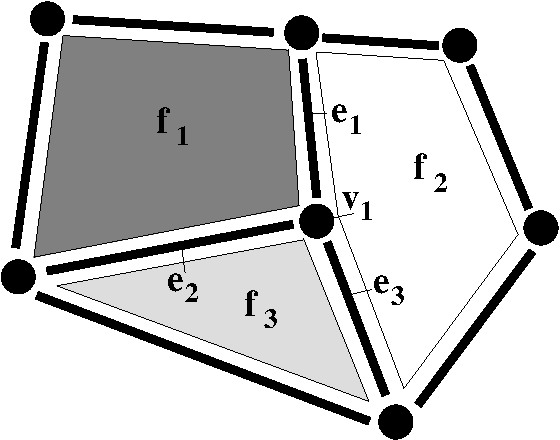
\includegraphics[width=.3\textwidth]
      {Combinatorial_map/fig/pdf/object2d}
      \qquad
      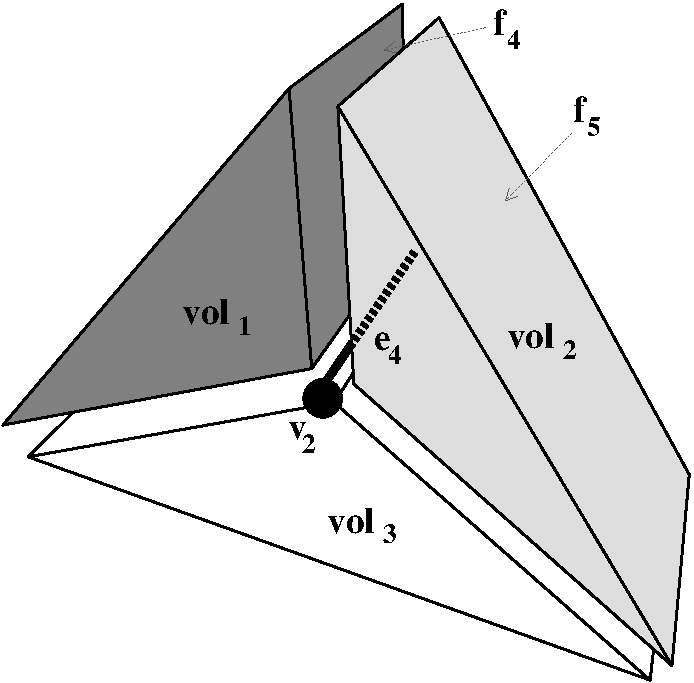
\includegraphics[width=.4\textwidth]
      {Combinatorial_map/fig/pdf/intuitif-example}
    \end{center}
  \end{ccTexOnly}
  \begin{ccHtmlOnly}
    <CENTER>
    <A HREF="fig/png/object2d.png"><img src="fig/png/object2d.png" alt=""></A>
    <A HREF="fig/png/intuitif-example.png"><img src="fig/png/intuitif-example.png" alt=""></A>
    </CENTER>
    \end{ccHtmlOnly}
    \caption{Example of subdivided objects that can be described by
      combinatorial maps.  \textbf{Left}: A 2D object composed of
      three facets (2-cells), named \emph{f1}, \emph{f2} and \emph{f3}, nine
      edges (1-cells) and seven vertices (0-cells).  \emph{f1} and
      \emph{f2} are adjacent along edge \emph{e1}, thus \emph{e1} is incident both
      to \emph{f1} and \emph{f2}. Vertex \emph{v1} is incident to edge \emph{e1}, thus
      \emph{v1} is incident to \emph{f1} and \emph{f2} by transitivity.
      \textbf{Right}: A 3D object (only partially represented for vertices and edges)
      composed of three volumes (3-cells), named \emph{vol1}, \emph{vol2}
      and \emph{vol3}, twelve facets (2-cells) (there is one facet
      \emph{f4} between \emph{vol1} and \emph{vol2}, and similarly between \emph{vol1}
      and \emph{vol3} and \emph{vol2} and \emph{vol3}), sixteen edges (1-cells),
      and eight vertices (0-cells). \emph{vol1} and \emph{vol2} are adjacent
      along facet \emph{f4}, thus \emph{f4} is incident both to \emph{vol1} and
      \emph{vol2}. Edge \emph{e4} is incident to the three facets between
      \emph{vol1} and \emph{vol2}, \emph{vol1} and \emph{vol3}, and \emph{vol2} and
      \emph{vol3}.  \emph{e4} is also incident to the three volumes by
      transitivity.}
    \label{fig-exemple-3Dmanifold}
\end{figure}

A combinatorial map is an edge-centered data structure describing the
cells and the incidence and adjacency relations, using only one basic
element called \emph{dart}, and a set of \emph{pointers} between these
darts.  A dart can be thought as a part of an oriented edge (1-cell),
together with a part of incident cells of dimensions 0, 2, 3,\ldots,
\emph{d}. When a dart \emph{d0} describes a part of an \cell{i} \emph{c}, we say that
\emph{d0} \emph{belongs} to \emph{c}, and that \emph{c} \emph{contains} \emph{d0}.  Let
us look at the example in Figure~\ref{fig-exemple-combi-maps} showing
the 2D and 3D combinatorial maps describing the two objects given in
Figure~\ref{fig-exemple-3Dmanifold}.
\begin{figure}[ht]
  \begin{ccTexOnly}
    \begin{center}
      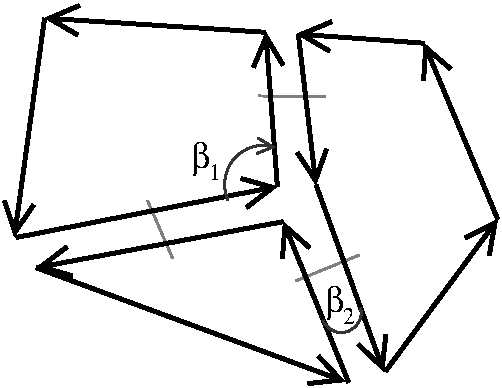
\includegraphics[width=.3\textwidth]
      {Combinatorial_map/fig/pdf/intuitif-example-map2d}
      \qquad
      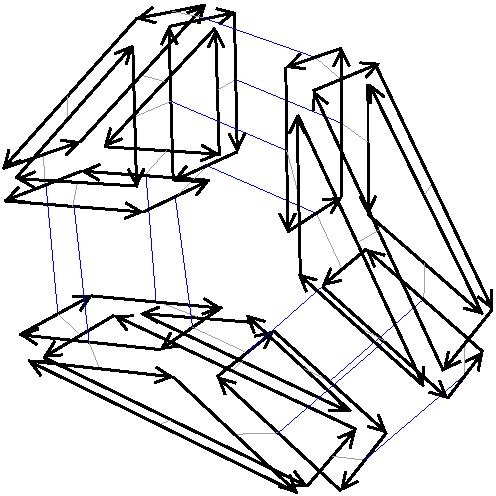
\includegraphics[width=.4\textwidth]
      {Combinatorial_map/fig/pdf/intuitif-example-map}
    \end{center}
  \end{ccTexOnly}
  \begin{ccHtmlOnly}
    <CENTER>
    <A HREF="fig/png/intuitif-example-map2d.png"><img src="fig/png/intuitif-example-map2d.png" alt=""></A>
    <A HREF="fig/png/intuitif-example-map.png"><img src="fig/png/intuitif-example-map.png" alt=""></A>
    </CENTER>
    \end{ccHtmlOnly}
    \caption{Combinatorial maps representing the objects given in 
      Figure~\ref{fig-exemple-3Dmanifold}.
      \textbf{Left}: The 2D combinatorial map which contains 12 darts.
      \textbf{Right}: The 3D combinatorial map which contains 54 darts
      (18 for each volume).
    }
    \label{fig-exemple-combi-maps}
\end{figure}

First let us start in 2D (Figure~\ref{fig-exemple-combi-maps} (Left)).
Facet \emph{f1} is described by four darts. These darts are linked
together with pointers. Starting from a dart and following a \betaun{} %\mbeta{1}
pointer, we get to a dart which belongs to the same facet but to the
next edge (1-cell, which explains the index~1 of~\betaun{}).
Starting from any dart and following \betaun{} pointers, we can reach
exactly all the darts describing the facet.  Starting from a dart and
following a \betadeux{} pointer, we get to a dart which belongs to the
same edge but to the neighboring facet (2-cell, which explains the
index~2 of~\betadeux{}).  Starting from any dart and following
\betadeux{} pointers, we can reach exactly all the darts describing the
edge (in 2D one or two darts).

Things are slightly different for vertices.  Indeed, each \betai{}
points to a dart belonging to a different \cell{i}, but also to a
different 0-cell (vertex).  This is so because two linked darts have
opposite orientations.  For this reason, starting from any dart
belonging to a vertex \emph{v}, we have to follow \betadeux{} then \betaun{}
to reach exactly the darts describing the vertex \emph{v}.  In fact, by
composing two \betai{}s, we always obtain a dart belonging to the
same vertex (if we do not start by following a \betaun{} pointer).

The main interest of combinatorial map definition based on darts and
\betai{} pointers is to be able to increase the dimension "only" by
adding new pointers. We can verify this fact by studying the 3D
example (Figure~\ref{fig-exemple-combi-maps} (Right)). In addition to
\betaun{} and \betadeux{} of the 2D case, there is a new pointer
\betatrois{}.

If we take a closer look at the central edge \emph{e4} shown in
Figure~\ref{fig-intuitive-exemple} (Left), we can see that it is
described by six darts linked together.  Starting from a dart and
following a \betatrois{} pointer, we get to a dart which belongs to the
same edge, to the same facet, but to the neighboring volume (a 3-cell,
which explains the index 3 in \betatrois{}).  Similarly, starting from
a dart and following a \betadeux{} pointer, we get to a dart which
belongs to the same edge, to the same volume, but to the neighboring
facet (2-cell). Starting from any of these six darts and following
\betadeux{} and \betatrois{} pointers, we can reach exactly the six darts
describing edge \emph{e4}.
%%%%%
\def\LargFig{.3\textwidth}
\begin{figure}
  \begin{ccTexOnly}
    \begin{center}
      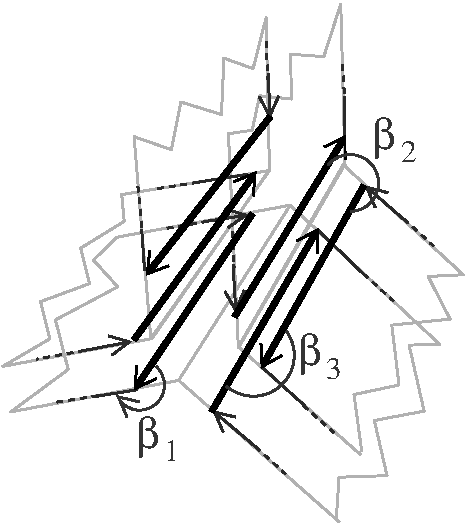
\includegraphics[width=\LargFig]{Combinatorial_map/fig/pdf/intuitif-example-zoom}
      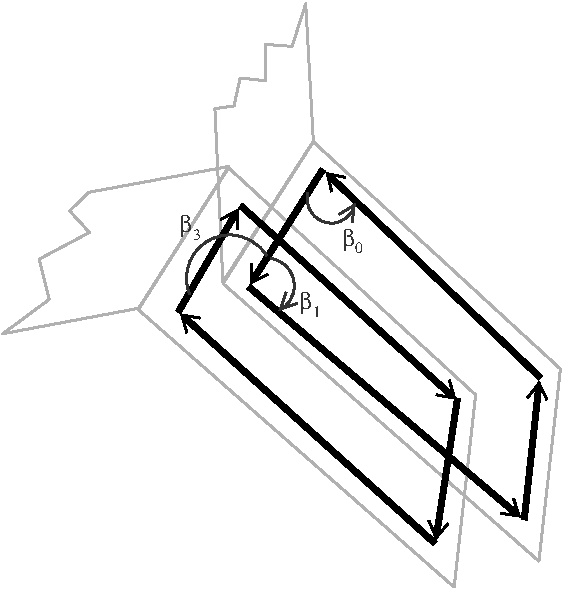
\includegraphics[width=\LargFig]{Combinatorial_map/fig/pdf/intuitif-example-zoom2}
    \end{center}
  \end{ccTexOnly}
  \begin{ccHtmlOnly}
    <CENTER>
    <!-- <A HREF="fig/png/intuitif-example-map.png">
    <img src="fig/png/intuitif-example-map.png" alt=""></A> -->
    <A HREF="fig/png/intuitif-example-zoom.png">
        <img src="fig/png/intuitif-example-zoom.png" alt=""></A>
    <A HREF="fig/png/intuitif-example-zoom2.png">
        <img src="fig/png/intuitif-example-zoom2.png" alt=""></A>
    </CENTER>
    \end{ccHtmlOnly}
    \caption{Two zooms on the 3D combinatorial map given in 
      Figure~\ref{fig-exemple-combi-maps} (Right).
      \textbf{Left}:~Zoom around the central edge \emph{e4} which details
      the six darts belonging to the edge.  \textbf{Right}:~Zoom
      around the facet between volumes \emph{vol2} and \emph{vol3} which
      details the eight darts belonging to the facet.}
    \label{fig-intuitive-exemple}
\end{figure}

For facets, by following a \betaun{} pointer, we get to a dart which
belongs to the same facet, to the same volume, but to the next edge
(1-cell, which explains the index~1 of~\betaun{}).  Starting from any
dart and following \betaun{} and \betatrois{} pointers, we can reach
exactly all the darts describing the facet (see
Figure~\ref{fig-intuitive-exemple} (Right)).
%
For volumes, starting from any dart and following \betaun{} and
\betadeux{} pointers, we can reach exactly all the darts describing the
volume.

For vertices, we have to follow \betadeux{} then \betaun{}, and
\betatrois{} then \betaun{} to reach exactly the darts describing the
vertex \emph{v}. Indeed, as in 2D, we have to compose two \betai{}s to
obtain a dart belonging to the same vertex (if we do not start by following a \betaun{} pointer).

In some cases, the general rule that by following a \betai{} we get a
dart which belongs to the neighboring \cell{i} is not true, as for example
for darts belonging to the boundary of the represented
object. For example, in Figure~\ref{fig-exemple-3Dmanifold} (Left), any dart
\emph{d0} that does not belong to edge \emph{e1}, \emph{e2} and \emph{e3}
belongs to a 2-cell, and there is no neighboring facet along the edge containing \emph{d0}.
Another example is in Figure~\ref{fig-exemple-3Dmanifold} (Right), for
any dart \emph{d0} that belongs to facet \emph{f5}.
\emph{d0} belongs to volume \emph{vol2}, but there is no neighboring volume
along this facet.  The general rule is also not true for unbounded
cells. For example if we remove a dart in
Figure~\ref{fig-exemple-combi-maps} (Left), we obtain an unbounded
facet having a dart without next dart for \betaun{}, and if we remove
a facet in Figure~\ref{fig-exemple-combi-maps} (Right), we obtain an
unbounded volume having some darts without neighboring facet for
\betadeux{}.  In such a case, there is a particular value called
$\varnothing$ used to describe that a dart \emph{d0} is not linked to
another dart in dimension~\emph{i}.

Combinatorial maps are defined in any dimension. A 0D combinatorial
map is a set of isolated darts describing isolated vertices. A 1D
combinatorial map describes paths or cycles of darts corresponding to
paths or cycles of edges, and equivalent to double linked lists.  The
most useful cases are 2D and 3D combinatorial maps. Since 2D
combinatorial maps are equivalent to halfedge data structure, notions
are illustrated in 3D in the following examples to help the reader 
understand this specific case. But it is important to keep in mind
that one main interest of combinatorial maps is their generic
definition in any dimension, and that everything presented in this
manual is valid in any dimension.

A \emph{d}D combinatorial map is useful when you want to describe \emph{d}D
objects and the adjacency relations between these objects, and you
want to be able to efficiency traverse these objects by using the
different relations.  For example, we can use a 3D combinatorial map
to describe a 3D segmented image: each 3-cell corresponds to a region
in the image and each 2-cell corresponds to a contact area between two
regions.

A combinatorial map does not contain any geometrical
information. However, this package allows to associate any information
to the cells of the combinatorial map. A specific information, which
is often used in practice, consists in adding linear geometry to a
combinatorial map by associating a point to each vertex of the
map\footnote{When an object has a point associated to each vertex,
  each edge is thus a straight line segment, which explains the name
  "linear geometry".}: this is the object of the
\ccc{Linear_cell_complex} package. This package can for example be
useful to describe 3D buildings as set of walls, rooms, doors and
windows (both combinatorial and geometrical descriptions) and all the
adjacency relations between these elements allowing for example to
move a camera in a given building from rooms to rooms by traversing
doors.

\section{Data Structure Presentation}\label{sec_presentation}

In this section, we describe \emph{d}D combinatorial maps in terms of data
structure and operations. Mathematical definitions are provided in
Section~\ref{sec_definition}, and a package description is given in
Section~\ref{sec-software-design}.

\subsection{Combinatorial Map and Darts}\label{ssec-combi-map-and-darts}

A \emph{d}D combinatorial map is a set of darts \emph{D}. A dart \emph{d0} is an
element that can be \emph{linked} with \emph{d}+1 darts by pointers called
\betai{}, with 0\myleq{}\emph{i}\myleq{}\emph{d}.  Dart \emph{d0} is said \emph{i-free}
when \betai{}(\emph{d0})=$\varnothing$.  Each \betai{}, for 2\myleq{}\emph{i}\myleq{}\emph{d},
is its own inverse, i.e., if dart \emph{d0} is not \emph{i}-free, then
\betai{}(\betai{}(\emph{d0}))=\emph{d0}.  This is different for \betazero{} and
\betaun{}: \betazero{} is the inverse of \betaun{}, i.e., if darts \emph{d1}
and \emph{d2} are such that \betaun{}(\emph{d1})=\emph{d2}, then
\betazero{}(\emph{d2})=\emph{d1}. Given dart \emph{d1}, if there is no dart \emph{d2} such
that \betaun{}(\emph{d2})=\emph{d1}, then \betazero{}(\emph{d1})=$\varnothing$.  $\varnothing$
is a constant, which does not belong to the set of darts \emph{D} of the
combinatorial map. However, by definition $\varnothing$ is linked with
itself for all \betai{}s: \myforall{}\emph{i}, 0\myleq{}\emph{i}\myleq{}\emph{d},
\betai{}($\varnothing)$=$\varnothing$.

A combinatorial map is \emph{without i-boundary} if there is no
\emph{i}-free dart, and it is \emph{without boundary} if it is without
\emph{i}-boundary for all dimensions 1\myleq{}\emph{i}\myleq{}\emph{d}.


We show in Figure~\ref{fig-exemple-carte3d} a 3D object and the
corresponding 3D combinatorial map.  This map has 40 darts represented
by arrows, some darts being numbered. In this combinatorial map, we
have for example \betaun{}(1)=2, \betadeux{}(1)=10, and
\betatrois{}(1)=5. This combinatorial map is without 1-boundary and
2-boundary, but has some 3-boundary, because some darts are 3-free,
for example \betatrois{}(10)=$\varnothing$ and \betatrois{}(12)=$\varnothing$.
%
\def\LargFig{.4\textwidth}
\begin{figure}
  \begin{ccTexOnly}
    \begin{center}
      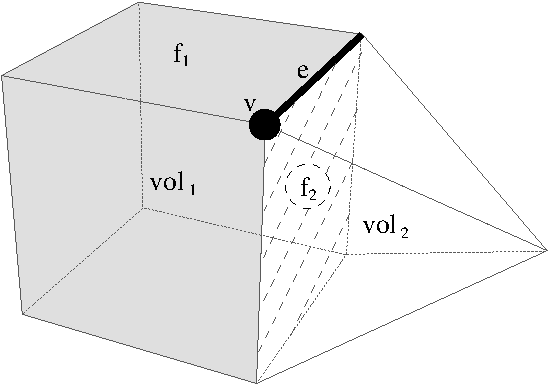
\includegraphics[width=\LargFig]{Combinatorial_map/fig/pdf/object3d}\qquad
      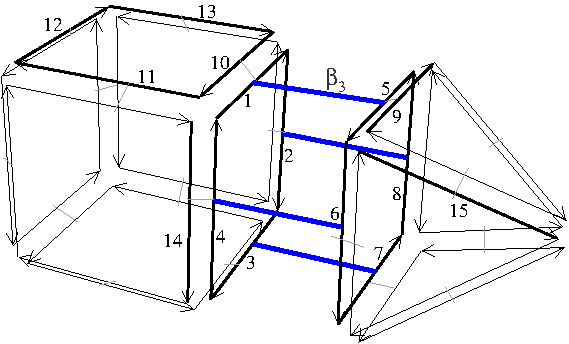
\includegraphics[width=\LargFig]{Combinatorial_map/fig/pdf/exemple-carte2-3d}
    \end{center}
  \end{ccTexOnly}
  \begin{ccHtmlOnly}
    <CENTER>
    <A HREF="fig/png/object3d.png">
    <img src="fig/png/object3d.png" alt=""></A>
    <A HREF="fig/png/exemple-carte2-3d.png">
        <img src="fig/png/exemple-carte2-3d.png" alt=""></A>
    </CENTER>
    \end{ccHtmlOnly}
    \caption{Example of a 3D combinatorial map. \textbf{Left}:~A 3D object
      made of two volumes adjacent along facet \emph{f2}. \textbf{Right}:~The
      corresponding 3D combinatorial map.  Darts are drawn with
      arrows, sometimes numbered.  Two darts linked by \betaun{} are
      drawn consecutively (for example \betaun{}(10)=11), and two
      darts linked by \betadeux{} are drawn parallel, in reverse
      orientations, with a little gray segment joining them (for
      example \betadeux{}(1)=10).  \betatrois{} pointers are represented by
      blue segments (for example \betatrois{}(1)=5).}
    \label{fig-exemple-carte3d}
\end{figure}

\subsection{Cells as Sets of Darts}\label{ssec-cells-in-map}

A cell in a \emph{d}D combinatorial map is implicitly represented by a
subset of darts.
In this section, we will see how to retrieve all cells containing a
given dart, how to retrieve all darts belonging to a cell containing a
given dart, and how incidence and adjacency relations are defined in
terms of darts.

The first important property of a combinatorial map is that
each dart belongs to an \cell{i}, \myforall{}\emph{i}, 0\myleq{}\emph{i}\myleq{}\emph{d}.
For example in 3D, a dart belongs to a vertex, an edge, a facet, and a
volume. This means that a 3D combinatorial map containing an isolated
dart contains exactly one vertex, one edge, one facet and one volume.

The second important property is that cells of a combinatorial map
correspond to specific \emph{orbits}.  Given a set 
\emph{S}\mysubseteq{}\{\betaun{},\myldots{},\betad{}\} and a dart
\emph{d0}, the \emph{orbit} \orbit{\emph{S}}(\emph{d0}) is the set of darts that can be
reached from \emph{d0} by following any combination of any \betai{}'s in \emph{S}
and their inverses (to simplify notations, we can use for example
\orbit{\betaun{},\betaquatre{}}(\emph{d0}) to denote \orbit{\emph{S}}(\emph{d0}) with
\emph{S}=\{\betaun{},\betaquatre{}\}).

Given a dart \emph{d0}, in general, \betai{}(\emph{d0}) (with 1\myleq{}\emph{i}\myleq{}d)
belongs to the same cells as \emph{d0}, only the \cell{i} and 0-cell are
different.  There are two exceptions: (1)~if \emph{d0} is \emph{i}-free, then
\betai{}(\emph{d0})=$\varnothing$; (2)~if \betai{}(\emph{d0}) belongs to the same \cell{i}
as \emph{d0} (case of multi-incidence). For example if an edge is an isolated
loop, it is incident twice to the same vertex, then given a dart \emph{d0}
belonging to this edge, \betaun{}(\emph{d0}) goes to the next edge, which is in
fact the same edge.

Since \betai{}(\emph{d0}) (with 1\myleq{}\emph{i}\myleq{}\emph{d}) allows to change the
current \cell{i}, all the darts that can be reached from \emph{d0} by
using any combination of \betaj{}'s, \myforall{}\emph{j}, 1\myleq{}\emph{j}\myleq{}\emph{d} and
\emph{j}\myneq{}\emph{i} and their inverse are contained in the same \cell{i} as
\emph{d0}.  The \cell{i} containing \emph{d0} is defined in terms of orbit by
\orbit{\betaun{},\myldots{},\betaimun{},\betaipun{},\myldots{},\betad{}}(\emph{d0}).

There is a special case for vertices. Given a dart \emph{d0}, the set of
darts contained in the same vertex as \emph{d0} are the darts that can be
reached from \emph{d0} by using any combination of \betai{}\comp{}\betaj{},
\myforall{}\emph{i},\emph{j}, 1\myleq{}\emph{i}\mylt{}\emph{j}\myleq{}\emph{d}, and their inverse.  The 0-cell
containing \emph{d0} is defined in terms of orbit by
\orbit{\{\betai{}\comp{}\betaj{}$|$\myforall{}\emph{i,j}: 1\myleq{}\emph{i}\mylt{}\emph{j}\myleq{}\emph{d}\}}(\emph{d0}).

Orbit \orbit{\betaun{},\myldots{},\betad{}}(\emph{d0}) is the \emph{connected
  component} containing dart \emph{d0}. A combinatorial map is
\emph{connected} if this set is equal to the set of all the darts
of the combinatorial map.

%AF: Je ne trouve pas ques les \forall s'integrent bien dans une phrase
%    et je preferais ceci: 
% A last important property of cells, is that for all dimensions i
% the set of \cells{i} form a partition of the set of darts D, i.e.
%
%    Je le dis ici a titre d'exemple, c'est a dire je recommende
%    que tu fasse un passe pour obtenir plus de ``phrases sans $..$''

A last important property of cells is that for all dimensions \emph{i} the
set of \cells{i} forms a partition of the set of darts \emph{D}, i.e.  for
any \emph{i}, the union of the sets of darts of all the \cells{i} is equal
to \emph{D}, and the sets of darts of two different \cells{i} are disjoint.

Let us give some examples of cells in 3D, for the 3D combinatorial map
of Figure~\ref{fig-exemple-carte3d}:
\begin{itemize}
\item All the darts belonging to the same edge can be obtained by any
  combination of \betadeux{} and \betatrois{}: for example edge \emph{e} of the
  object corresponds in the combinatorial map to the set of darts
  \{1,5,9,10\}. Given any dart belonging to this edge, we retrieve
  all the other darts by, for example, a breadth-first traversal. In terms
  of orbits, this 1-cell corresponds to \orbit{\betadeux{},\betatrois{}}(1).

\item All the darts belonging to the same facet can be obtained by any
  combination of \betaun{} and \betatrois{}: for example facet \emph{f2}
  corresponds in the combinatorial map to the set of darts
  \{1,2,3,4,5,6,7,8\}. Facet \emph{f1} corresponds to the set of darts
  \{10,11,12,13\}. Note that these last darts are 3-free since
  there is no other volume sharing this facet.  In terms of orbits,
  \emph{f2} corresponds to \orbit{\betaun{},\betatrois{}}(1) and \emph{f1}
  corresponds to \orbit{\betaun{},\betatrois{}}(10).

\item All the darts belonging to the same volume can be obtained by
  any combination of \betaun{} and \betadeux{}: for example volume \emph{vol1}
  corresponds in the combinatorial map to the set of the twenty-four
  darts representing the cube. In terms of orbits, \emph{vol1} corresponds
  to \orbit{\betaun{},\betadeux{}}(1).

\item All the darts belonging to the same vertex can be obtained by
  any combination of \betaun{}\comp{}\betadeux{},
  \betaun{}\comp{}\betatrois{} and \betadeux{}\comp{}\betatrois{} and their inverse
  functions.  In our example, vertex \emph{v} of the object corresponds
  in the combinatorial map to the set of darts \{1,6,9,11,14,15\}.
  Starting from dart 1, we obtain for example dart
  14=(\betaun{}\comp{}\betadeux{})\ccTexHtml{$^{-1}$}{<sup>-1</sup>}(1)=\betadeux{}\comp{}\betazero{}(1), dart
  11=\betaun{}\comp{}\betadeux{}(1), and dart 9=\betadeux{}\comp{}\betatrois{}(1).
  Intuitively, the set of darts corresponding to a vertex contains all
  the darts represented by arrows starting from this vertex.  In terms
  of orbits, \emph{v} corresponds to \orbit{\betaun{}\comp{}\betadeux{},
    \betaun{}\comp{}\betatrois{}, \betadeux{}\comp{}\betatrois{}}(1).
\end{itemize}

Using this definition of cells as sets of darts, we can retrieve all the
incidence and adjacency relations between the cells of the subdivision
in a combinatorial map.  Two cells are \emph{incident} if the
intersection of their two sets of darts is non empty (whatever the
dimension of the two cells). Two \cells{i} \emph{c1} and \emph{c2}, 
1\myleq{}\emph{i}\myleq{}\emph{d}, are \emph{adjacent} if there is 
\emph{d1}\myin{}\emph{c1} and \emph{d2}\myin{}\emph{c2} such that
\emph{d1}=\betai{}(\emph{d2}) (or \emph{d2}=\betai{}(\emph{d1}) 
for \emph{i}=1).

In the example of Figure~\ref{fig-exemple-carte3d}, vertex \emph{v} and
edge \emph{e} are incident since the intersection of the two corresponding
sets of darts is \{1,9\}\myneq{}\myemptyset{}. Vertex \emph{v} is incident to facet
\emph{f2} since the intersection of the two corresponding sets of darts is
\{1,6\}\myneq{}\myemptyset{}. Edge \emph{e} and facet \emph{f1} are incident
since the intersection of the two corresponding sets of darts is
\{10\}\myneq{}\myemptyset{}. Finally, facets \emph{f1} and \emph{f2} are adjacent
because 10\myin{}\emph{f1}, 1\myin{}\emph{f2} and 10=\betadeux{}(1).

We can consider \cells{i} in a dimension \emph{d'} with  \emph{i}\myleq{}\emph{d'}\myleq{}
\emph{d}. The idea is to consider the \cells{i} as if the combinatorial map
was in \emph{d'} dimension. For that, we only take into account the
\betaj{}s for \emph{j}\myleq{}\emph{d'}.  The \cell{i} containing \emph{d0} in dimension
\emph{d'} is the orbit
\orbit{\betaun{},\myldots{},\betaimun{},\betaipun{},\myldots{},\betadprim{}}(\emph{d0}), and 
the 0-cell is the orbit \orbit{\{\betai{}\comp{}\betaj{}$|$\myforall{}\emph{i,j}: 
2\myleq{}\emph{i}\mylt{}\emph{j}\myleq{}\emph{d'}\}}(\emph{d0}).  By default, \cells{i} are considered in
dimension \emph{d}, the dimension of the combinatorial map.

In the example of Figure~\ref{fig-exemple-carte3d}, the 2-cell
containing dart 1 is facet \emph{f2} which is the set of darts
\{1,2,3,4,5,6,7,8\}. If we consider the same 2-cell in dimension~2,
we obtain the set of darts \{1,2,3,4\}. Intuitively we "forget"
\betatrois{} and we obtain the set of darts of the facet containing dart
1 restricted to the volume containing this dart.

\subsection{How to Associate Information to Cells}
\label{ssec-associate-attributes}

Combinatorial maps only describe the cells of the subdvision, and all
the incidence and adjacency relations between these cells. This is not
enough for many applications which need to associate
\emph{information} to cells.  This can be geometric or non-geometric
information, such as 3D points associated to vertices, the edge length
associated to edges, or a color or normal to a facet.

To answer this need, a combinatorial map allows to create
\emph{attributes} which are able to store any information, and to
associate attributes to cells of the combinatorial map.  We denote
\emph{i}-attributes for the attributes associated with
\cells{i}. Attributes may exist for only some of the dimensions, and
if they exist for dimension \emph{i}, they do not necessarily exist for
each of the \cells{i}.  More precisely, \emph{i}-attributes are associated
to \cells{i} by an injection:
\begin{itemize}
\item two different \cells{i} are associated to two different
  \emph{i}-attributes;
\item an \cell{i} may have no associated \emph{i}-attribute.
\end{itemize}

Since \cells{i} are not explicitely represented in combinatorial maps,
the association between \cells{i} and \emph{i}-attributes is transferred to
darts: if attribute \emph{a} is associated to \cell{i} \emph{c}, all the darts
belonging to \emph{c} are associated to \emph{a}.

We can see two examples of combinatorial maps having some
attributes in Figure~\ref{fig-exemple-attribs}. In the first example
(Left), a 2D combinatorial map has 1-attributes containing a float,
for example corresponding to the length of the associated 1-cell, and
2-attributes containing a color in RGB format.  In the second example
(Right), a 3D combinatorial map has 2-attributes containing a color
in RGB format.
%
\begin{figure}
  \begin{ccTexOnly}
    \begin{center}
      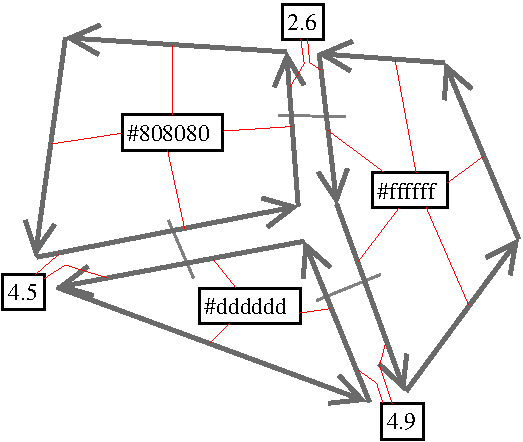
\includegraphics[width=.3\textwidth]{Combinatorial_map/fig/pdf/map2d-with-attrib}\qquad
      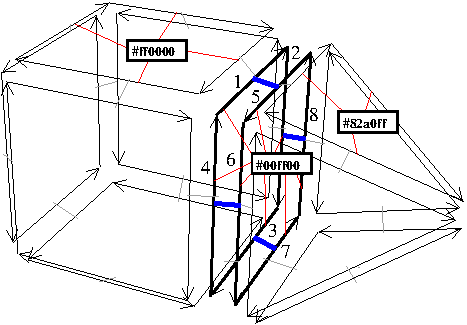
\includegraphics[width=.45\textwidth]{Combinatorial_map/fig/pdf/exemple-carte-3d-sew2}
    \end{center}
  \end{ccTexOnly}
  \begin{ccHtmlOnly}
    <CENTER> <A HREF="fig/png/map2d-with-attrib.png"> <img
    src="fig/png/map2d-with-attrib.png" alt=""></A> <A
    HREF="fig/png/exemple-carte-3d-sew2.png"> <img
    src="fig/png/exemple-carte-3d-sew2.png" alt=""></A> </CENTER>
  \end{ccHtmlOnly}
  \caption{Example of combinatorial maps with attributes. Attributes
    are represented by black rectangles containing an information, and
    association between darts and attributes are represented by small
    lines.  \textbf{Left}:~A 2D combinatorial map with 1-attributes
    containing a double, for example corresponding to the length of
    the 1-cell, and 2-attributes containing a color in RGB format.
    Only three edges of the combinatorial map, among the nine, are
    associated to a 1-attribute. All the 2-cells are associated to a
    2-attribute. \textbf{Right}:~A 3D combinatorial map with
    2-attributes containing a color in RGB format. Only three 2-cells
    of the combinatorial map, among the ten, are associated to a
    2-attribute.}
  \label{fig-exemple-attribs}
\end{figure}

\subsection{Combinatorial Map Properties}\label{ssec-combimap-validity}

There are some conditions that a combinatorial map must satisfy to be
valid. Some of them have already been given about the \betats{} pointers
(see Section~\ref{ssec-combi-map-and-darts}) and about the association
between darts and attributes (see
Section~\ref{ssec-associate-attributes}).

There is an additional condition related to the type of represented
objects, which are \emph{quasi-manifold} orientable \emph{d}D objects.  A
\emph{d}D quasi-manifold is an object obtained by taking some isolated
\cells{d}, and allowing to glue \cells{d} along \cells{(d-1)}. It is
orientable if it is possible to embed it in the Euclidean space and to
define a global "left" and "right" direction in each point of the
embedded object.  In 2D, quasi-manifolds are manifolds, but this is no
longer true in higher dimension as we can see in the example presented
in Figure~\ref{fig-quasivariete}.  In this example, the object to the
right is not a manifold since the neighborhood of the point \emph{p} in the
object is not homeomorphic\footnote{Intuitively, two objects are
  homeomorphic if each object can be continuously deformed into the
  second one.  In such a case, the two objects have exactly the same
  topological properties.}  to a 3D ball.
%
%%%%%%%%%%%%%%%%%%%%%%%%%%%%%% FIGURE %%%%%%%%%%%%%%%%%%%%%%%%%%%%%%%%%%
\begin{figure}
  \begin{ccTexOnly}
    \begin{center}
    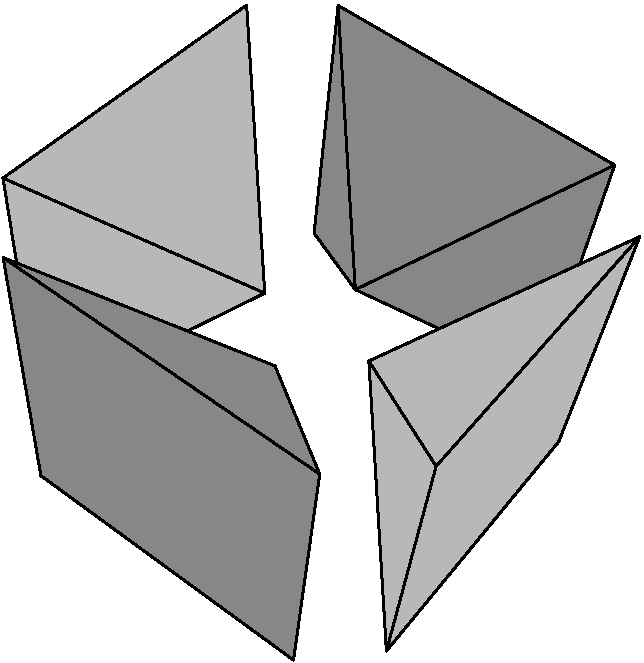
\includegraphics[width=.33\textwidth]{Combinatorial_map/fig/pdf/quasivarietea}
    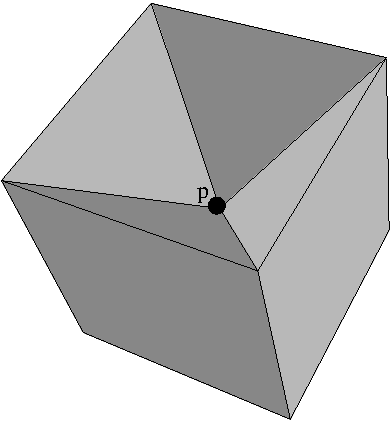
\includegraphics[width=.33\textwidth]{Combinatorial_map/fig/pdf/quasivariete}
    \end{center}
  \end{ccTexOnly}
  \begin{ccHtmlOnly}
    <CENTER>
    <A HREF="fig/png/quasivarietea.png"><img src="fig/png/quasivarietea.png" alt=""></A>
    <A HREF="fig/png/quasivariete.png"><img src="fig/png/quasivariete.png" alt=""></A>
    </CENTER>
  \end{ccHtmlOnly} 
  \caption{Example of a 3D quasi-manifold which is not a manifold.
    The object to the right is made of the four pyramids (shown to the
    left) glued together along facets, thus it is a quasi-manifold.}
  \label{fig-quasivariete}
\end{figure}
%%%%%%%%%%%%%%%%%%%%%%%%%%%%%%%%%%%%%%%%%%%%%%%%%%%%%%%%%%%%%%%%%%%%%%%%

Combinatorial maps can only represent quasi-manifolds due to the
definition of \betats{} pointers. As we have seen in
Section~\ref{ssec-cells-in-map}, \betai{}(\emph{d0}) (with 1\myleq{}\emph{i}\myleq{}\emph{d})
belongs to the same cells as \emph{d0}, only the \cell{i} and 0-cell are
different. In other words, \betai{} links two \cells{i} that
share a common \cell{(i-1)}: it is not possible to link more than two
\cells{i} along a same \cell{(i-1)}.
For this reason, it is not possible to describe non quasi-manifold
objects as those shown in Figure~\ref{fig-nonquasi-manifold} by
combinatorial maps.
%
%%%%%%%%%%%%%%%%%%%%%%%%%%%%%%%%%%%%%%%%%%%%%%%%%%%%%%%%%
\begin{figure}[ht]
  \begin{ccTexOnly}
    \begin{center}
      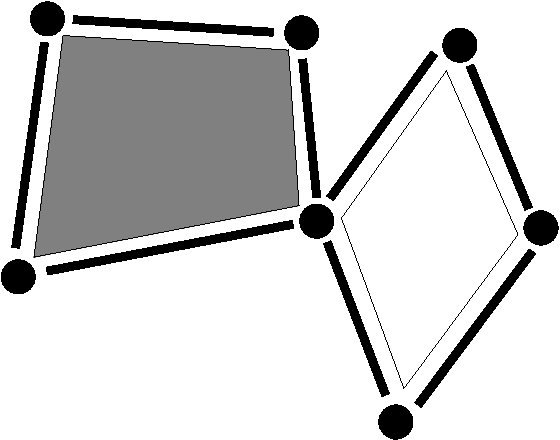
\includegraphics[width=.22\textwidth]
      {Combinatorial_map/fig/pdf/object2d-nonmanifold}
      \qquad
      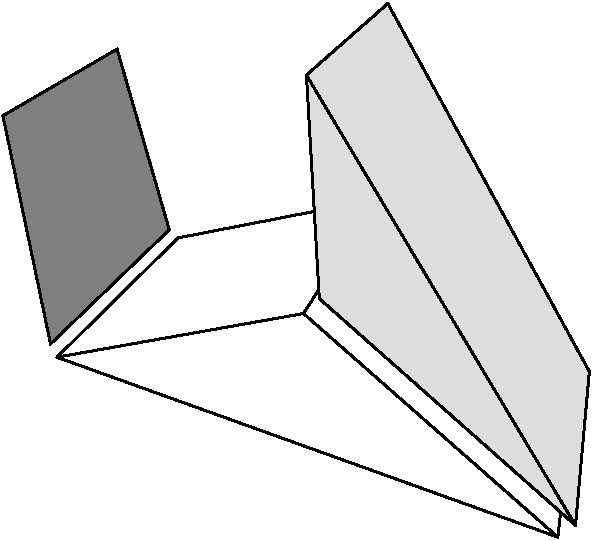
\includegraphics[width=.3\textwidth]
      {Combinatorial_map/fig/pdf/object3d-nonmanifold}
      \qquad
      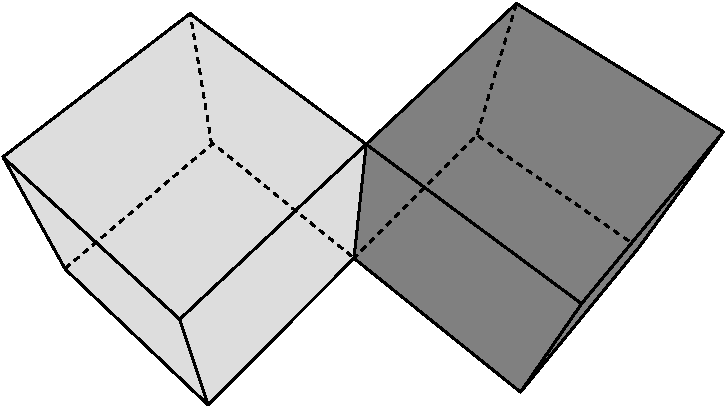
\includegraphics[width=.35\textwidth]
      {Combinatorial_map/fig/pdf/object3d-nonmanifold2}
    \end{center}
  \end{ccTexOnly}
  \begin{ccHtmlOnly}
    <CENTER>
    <A HREF="fig/png/object2d-nonmanifold.png"><img src="fig/png/object2d-nonmanifold.png" alt=""></A>
    <A HREF="fig/png/object3d-nonmanifold.png"><img src="fig/png/object3d-nonmanifold.png" alt=""></A>
    <A HREF="fig/png/object3d-nonmanifold2.png"><img src="fig/png/object3d-nonmanifold2.png" alt=""></A>
    </CENTER>
    \end{ccHtmlOnly}
    \caption{Three examples of non quasi-manifold
      objects. \textbf{Left}: A 2D object which is not a
      quasi-manifold since the two 2-cells share a common vertex but
      no common 1-cell.  \textbf{Middle}: A 3D object which is not a
      quasi-manifold since is it not only composed by 3D cells glued
      together (there is an isolated 2-cell in dark
      gray). \textbf{Right}: A 3D object which is not a quasi-manifold
      since the two 3-cells share a common edge but no common 2-cell.
    }
    \label{fig-nonquasi-manifold}
\end{figure}
%%%%%%%%%%%%%%%%%%%%%%%%%%%%%%%%%%%%%%%%%%%%%%%%%%%%%%%%%

Due to this additional condition, any objects can not be represented
by a combinatorial map but only orientable quasi-manifolds. We need to
study now the inverse relation. Does any set of darts linked together by
\betai{}'s, with 0\myleq{}\emph{i}\myleq{}\emph{d} correspond to a quasi-manifold?  As
we can see in Figure~\ref{fig-pb-carte}, the answer is no.
%
%%%%%%%%%%%%%%%%%%%%%%%%%%%%%%%%%%%%%%%%%%%%%%%%%%%%%%%%%
\begin{figure}[ht]
  \begin{ccTexOnly}
    \begin{center}
      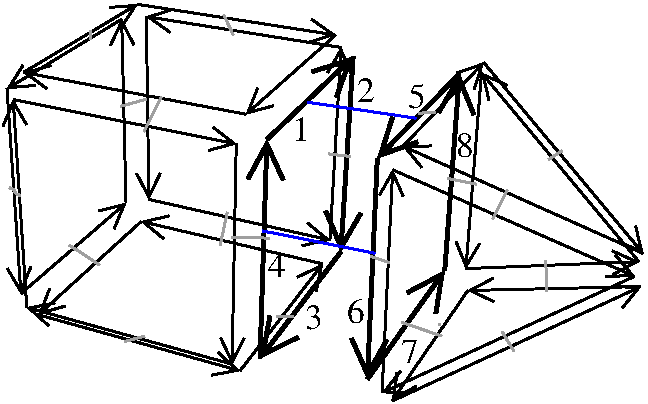
\includegraphics[width=.4\textwidth]
      {Combinatorial_map/fig/pdf/pb-carte3D}
      \qquad
      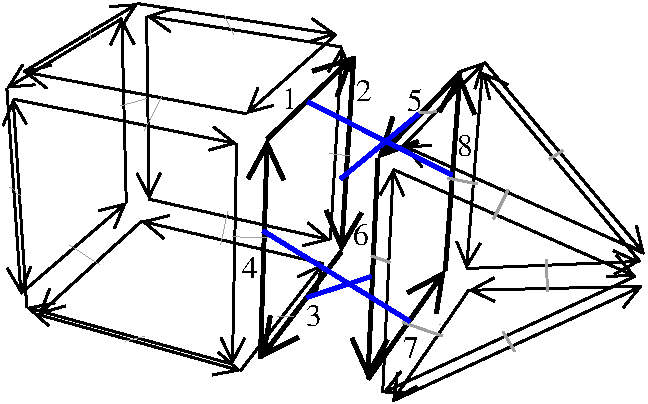
\includegraphics[width=.4\textwidth]
      {Combinatorial_map/fig/pdf/pb2-carte3D}
    \end{center}
  \end{ccTexOnly}
  \begin{ccHtmlOnly}
    <CENTER>
    <A HREF="fig/png/pb-carte3D.png"><img src="fig/png/pb-carte3D.png" alt=""></A>
    <A HREF="fig/png/pb2-carte3D.png"><img src="fig/png/pb2-carte3D.png" alt=""></A>
    </CENTER>
    \end{ccHtmlOnly}
    \caption{Two examples of darts linked together by some \betazero{},
      \betaun{}, \betadeux{} and \betatrois{} which does not represent a 3D
      quasi-manifold, and thus which are not 3D combinatorial map. 
      \textbf{Left}: In this example, all the darts are 3-free except
      \betatrois{}(1)=5 and \betatrois{}(4)=6 (and vice-versa).
      \textbf{Right}: In this example, darts linked by \betatrois{} 
      are not in the same order in both 3-cells.
    }
    \label{fig-pb-carte}
\end{figure}
%%%%%%%%%%%%%%%%%%%%%%%%%%%%%%%%%%%%%%%%%%%%%%%%%%%%%%%%%

In the first example (Left), there are two 3-cells (one to the left
for the cube, a second to the right for the pyramid) which are
"partially adjacent" along one 2-cell. Indeed, only two darts
of the 2-cell are linked by \betatrois{}. We have \betatrois{}(1)=5 and
\betatrois{}(4)=6 (and reciprocally).  This configuration is not possible
in a quasi-manifold: two \cells{d} are always glue along an "entire"
\cells{(d-1)}.

But as we can see in the second example (Right), the condition that
all the darts of the cell are linked in not sufficient. Indeed, in
this example, all the darts of the 2-cell between the cube and the
pyramid are linked together by \betatrois{}. However, this configuration
does not correspond to an orientable 3D quasi-manifold. Indeed, the
operation of gluing two \cells{d} along one \cell{(d-1)} must
preserve the initial \cell{(d-1)}.

To avoid these two kinds of configurations, conditions are added on
\betats{} pointers compositions (see Section~\ref{sec_definition},
condition~(4) of the definition of combinatorial maps). Intuitively
these conditions say that if two darts are linked by \betai{}, then
all the required darts are linked by \betai{} two by two in such a
way that neighborhood relations are preserved.


We say that a combinatorial map is \emph{valid} if it satisfies all
the conditions on \betats{} pointers and on association between darts
and attributes.  High level operations provided on combinatorial maps
ensure that these conditions are always satisfied. Sometimes, it can
be useful to use low level operations in a specific algorithm, for
example to modify locally a combinatorial map in a really fast way. In
such a case, additional operations may be needed to restore these
validity conditions.


\section{Software Design}\label{sec-software-design}

The diagram in Figure~\ref{fig-diagram_class} shows the different
classes of the package.  \ccc{Combinatorial_map} is the main class
(see Section~\ref{ssec-combinatorial-map}). It allows to manage darts
(see Section~\ref{ssec-darts}) and attributes (see
Section~\ref{ssec-attributes}).
Users can customize a combinatorial map thanks to an items class (see
Section~\ref{ssec-item}), which defines the dart type and the
attribute types. These types may be different for different
dimensions, and they may also be void.  The darts and attributes are
accessed through \emph{handles}. A handle is a model of the
\ccc{Handle} concept, thus supporting the two dereference operators
\ccc{operator*} and \ccc{operator->}.

\begin{figure}
  \begin{ccTexOnly}
    \begin{center}
      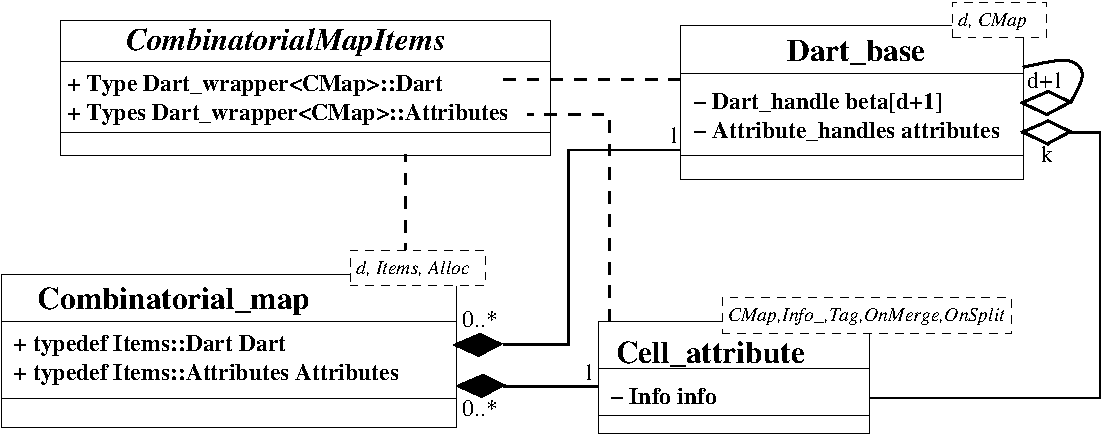
\includegraphics[width=.95\textwidth]
      {Combinatorial_map/fig/pdf/Diagramme_class}
    \end{center}
  \end{ccTexOnly}
  \begin{ccHtmlOnly}
    <CENTER>
    <A HREF="fig/png/Diagramme_class.png">
        <img src="fig/png/Diagramme_class.png" alt=""></A>
    </CENTER>
    \end{ccHtmlOnly}
    \caption{UML diagram of the main classes of the package. \emph{k} is the number of
      non void attributes.}
    \label{fig-diagram_class}
\end{figure}

\subsection{Combinatorial Maps}\label{ssec-combinatorial-map}

The class \ccc{Combinatorial_map<d,Items,Alloc>} is a model of the
\ccc{CombinatorialMap} concept.  It has three template parameters
standing for the dimension of the combinatorial map (an 
\ccc{unsigned int}), an items class (a model of the 
\ccc{CombinatorialMapItems}
concept), and an allocator which must be a model of the allocator
concept of the {\stl}.  Default classes are provided for the items and
the allocator classes.

The main role of the class \ccc{Combinatorial_map} is the storage and
the management of darts. It allows to create or remove an isolated
dart from the combinatorial map.  The \ccc{Dart_handle} type defines a
handle to the type of used darts (given in the items class).
\ccc{Combinatorial_map} provides several \emph{ranges} which allow to
iterate over specific subsets of darts of the combinatorial map (see
Section~\ref{ssec-range}).  It also defines several methods to link
and to unlink darts by \betai{}s (see
Section~\ref{ssec-link-darts}). We said that a dart \emph{d0} is \emph{i}-free 
if \betai{}(\emph{d0})=$\varnothing$.   The $\varnothing$ constant is
represented in the class \ccc{Combinatorial_map} through a 
\ccc{static const Dart_handle} 
called \nulldart{}.  Finally, some high level
operations are defined as global functions taking a
\ccc{Combinatorial_map} as argument (see
Section~\ref{ssec-operations})

The second role of the class \ccc{Combinatorial_map} is the storage
and the management of attributes.  It allows to create or remove an
attribute, and provides methods to associate attributes and cells.
A range is defined for each \emph{i}-attribute allowing to iterate
over all the \emph{i}-attributes of the combinatorial map.  Finally,
\ccc{Combinatorial_map} defines several types allowing to manage the
attributes. We can use
\ccc{Combinatorial_map::Attribute_handle<i>::type} for a handle to the
\emph{i}-attributes (and the const version
\ccc{Combinatorial_map::Attribute_const_handle<i>::type}) and
\ccc{Combinatorial_map::Attribute_type<i>::type} for the type of the
\emph{i}-attributes.

\subsection{Combinatorial Map Items}\label{ssec-item}

The \ccc{CombinatorialMapItems} concept defines dart and attribute
types of a combinatorial map. It contains one inner class named
\ccc{Dart_wrapper}, having one template parameter, \ccc{CMap}, a model
of \ccc{CombinatorialMap} concept.  The \ccc{Dart_wrapper<CMap>} class
provides two local types: \ccc{Dart} which must be a model of the
\ccc{Dart} concept, and \ccc{Attributes} which defines the attributes
and their types.

The \ccc{Attributes} tuple must contain at most \emph{d}+1 types (one for
each possible cell dimension of the combinatorial map).  Each type of
the tuple must be either a model of the \ccc{CellAttribute} concept or
\ccc{void}.  The first type corresponds to 0-attributes, the second to
1-attributes and so on. If the \ccTexHtml{$i^{\mbox{th}}$}{i<sup>th</sup>} type in the tuple is  
\ccc{void}, \emph{(i-1)}-attributes are disabled: we say that
\emph{(i-1)}-attributes are \emph{void}.  Otherwise, \emph{(i-1)}-attributes are
enabled and have the given type: we say \emph{(i-1)}-attributes are
\emph{non void}.  If the size of the tuple is \emph{k}, with \emph{k}\mylt{}\emph{dimension+1}, \myforall{}\emph{i}: \emph{k}\myleq{}\emph{i}\myleq{}dimension, 
\emph{i}-attributes are void.

The class \ccc{Combinatorial_map_min_items<d>} is a model of the
\ccc{CombinatorialMapItems} concept which can be used for default behaviors.
It defines \ccc{CGAL::Dart<d,CMap>} as type of dart, and
\ccc{Attributes} as empty tuple.

\subsection{Darts}\label{ssec-darts}

The class \ccc{Dart<d,CMap>}, a model of the \ccc{Dart} concept,
defines a \emph{d}D dart. It has two template parameters standing for the
dimension of the combinatorial map, and a model of the
\ccc{CombinatorialMap} concept, which provides the two types
\ccc{Dart_handle} and \ccc{Dart_const_handle}. 

Each instance \ccc{d0} of \ccc{Dart<d,CMap>} stores the \betai{} pointers in an
array of \emph{d}+1 \ccc{Dart_handle} (because we describe also the
\betazero{} pointer).  It also stores the attributes associated to this
dart in a tuple of \ccc{CMap::Attribute_handle<i>::type}, one for each
non void \emph{i}-attribute.

Methods are defined allowing to retrieve each \betai{} and each
associated \emph{i}-attribute of \ccc{d0}, and allowing to test if \ccc{d0}
dart is \emph{i}-free.

Note that the use of the \ccc{Dart} class is not hard wired in
the combinatorial map class. Users can provide their own model of the
\ccc{Dart} concept, and pass it to the combinatorial map with the help
of a custom item class.

\subsection{Cell Attributes}\label{ssec-attributes}

The class \ccc{Cell_attribute<CMap,Info_,Tag,OnMerge,OnSplit>}, a
model of the \ccc{CellAttribute} concept, represents an attribute
associated with a cell of a combinatorial map.  The 
template parameter \ccc{CMap} must be a model of the
\ccc{CombinatorialMap} concept.  The attribute stores a handle to one
dart of its associated cell when the template parameter \ccc{Tag} is
\ccc{Tag_true}.
\ccc{Info_} is the type of information stored in the attribute. It may
be \ccc{void}.  \ccc{OnMerge} and \ccc{OnSplit} must be either
\ccc{Null_functor}, or models of the \ccc{Binary Function} concept
having two references to a model of \ccc{CellAttribute} as type of
both parameters and \ccc{void} as return type.  There are two default
parameters for \ccc{OnMerge} and \ccc{OnSplit}, which are
\ccc{Null_functor}, a default parameter for \ccc{Tag} which is
\ccc{Tag_true}, and a default parameter for \ccc{Info_} which is
\ccc{void}.

If \ccc{Info_} is different from \ccc{void}, the class
\ccc{Cell_attribute} contains two methods \ccc{info()} returning the
information contained in the attribute (const and non const version).
The information is returned by reference, thus the non const version
allows the modification of the information.

Two attributes are merged when their corresponding cells are merged
into one cell during some operation. In this case, the functor
\ccc{OnMerge} is called, unless it is equal to \ccc{Null_functor}.
This functor allows the user to define its own custom behavior when
two attributes are merged (for example if the information is a color,
we can compute the average color of the two initial attributes, and
affect this value to the first attribute, see example in
Section~\ref{ssec-combi-map-with-color}).  Similarly, the functor
\ccc{OnSplit} is called when one attribute is split in two, because
its corresponding cell is split in two during some operation, unless
it is equal to \ccc{Null_functor}.  In any high level operation,
\ccc{OnMerge} is called before to start the operation (i.e. before
modifying the combinatorial map), and \ccc{OnSplit} is called when the
operation is finished (i.e. after all the modifications were made).

What we said for the dart also holds for the cell attribute.  The
combinatorial map can be used with any user defined model of the 
\ccc{CellAttribute} concept.

\subsection{Example of Combinatorial Map Definition}\label{ssec-example-def}

Here comes an example of two combinatorial map definitions.  The first
case \ccc{Example_cmap4} defines a 4D combinatorial map which uses all
the default values (\ccc{Dart} and
\ccc{Combinatorial_map_min_items}). The second example
\ccc{Example_custom_cmap3} uses its own model of the
\ccc{CombinatorialMapItems} concept. In this model, the type
of dart is \ccc{Dart<3,CMap>}, thus a dart is in 3D, and an
attribute containing an integer is associated to edges.

\begin{ccExampleCode}
typedef CGAL::Combinatorial_map<4> Example_cmap4;

struct Example_items_3
{
   template <class CMap>
   struct Dart_wrapper
   {
     typedef CGAL::Dart<3, CMap> Dart;
     typedef CGAL::Cell_attribute<CMap, int> Edge_attrib;
     typedef CGAL::cpp0x::tuple<void,Edge_attrib> Attributes;
   };
};
typedef CGAL::Combinatorial_map<3, Example_items_3> Example_custom_cmap3;
\end{ccExampleCode}


\section{Iteration and Creation Operations}

An important operation in combinatorial maps consists in iterating
over specific subsets of darts or over attributes. For that, several
\emph{ranges} are offered (see Section~\ref{ssec-range}).  A range is
a model of the \ccc{Range} concept, thus supporting the two methods
\ccc{begin()} and \ccc{end()} allowing to iterate over all the
elements in the range.  Several global functions allow to create
specific configurations of darts into a combinatorial map (see
Section~\ref{ssec-construction}).  Darts can be marked during
operations, for example when performing a breadth-first search
traversal, thanks to Boolean marks (see
Sections~\ref{ssec-adv-marks}).  In the following, we denote by
\ccc{dh0}, \ccc{dh1}, \ccc{dh2} the dart handles for the darts
\ccc{d0}, \ccc{d1}, \ccc{d2}, respectively. That is \ccc{d0 == *dh0}.

\subsection{Iterating over Orbits, Cells, and Attributes}\label{ssec-range}

The combinatorial map offers iterators to traverse the darts
of a specific orbit, to traverse all darts of one cell, or
one dart per cell, and to traverse all \emph{i}-attributes.

Instead of the \ccc{begin()/end()} member function pair as we know it
from \stl\ containers, and from most \cgal\ data structures, the
combinatorial map defines range classes which are all models of the
\ccc{Range} concept.

There are three different categories of dart range classes:
\begin{itemize}
\item \ccc{Dart_range}: range of all the darts of a combinatorial map;
\item \ccc{Dart_of_orbit_range<Beta...>}: range of all the darts of
  the orbit \orbit{\ccc{Beta...}}(\emph{d0}) for a given \emph{d0}.  \ccc{Beta...} is a
  sequence of integers 
  \ccTexHtml{$i_1$}{i<sub>1</sub>},\myldots{},\ccTexHtml{$i_k$}{i<sub>k</sub>}, 
  each \ccTexHtml{$i_j$}{i<sub>j</sub>}\myin{}\{0,\ldots,\emph{d}\}. 
  These integers must satisfy:
  \ccTexHtml{$i_1$}{i<sub>1</sub>}\mylt{}\ccTexHtml{$i_2$}{i<sub>2</sub>}\mylt{}\myldots{}\mylt{}\ccTexHtml{$i_k$}{i<sub>k</sub>},
  and (\ccTexHtml{$i_1$}{i<sub>1</sub>}\myneq{}0 or \ccTexHtml{$i_2$}{i<sub>2</sub>}\myneq{}1) 
  (for example \ccc{Dart_of_orbit_range<1,2>} for the orbit
  \orbit{\betaun{},\betadeux{}}(\emph{d0}));	
\item \ccc{Dart_of_cell_range<i,dim>}: range of all the darts of
  the \cell{i} containing a given dart. The \cell{i} is considered in
  dimension \ccc{dim} (with 0\myleq{}\emph{dim}\myleq{}\emph{d}, 
  \emph{dim}=\emph{d} by default), 
  with 0\myleq{}\emph{i}\myleq{}\emph{dim+1}. If \emph{i}=\emph{dim+1},
  \ccc{Dart_of_cell_range<i,dim>} is the range of all the darts of
  the connected component containing a given dart.
\end{itemize}

There are also two different classes of ranges containing one dart per
\cell{i}. Note that in these classes, the dart of each \cell{i} can
be any dart of the cell. Moreover, each \cell{i} (and \cell{j} in the
second case) is considered in dimension \ccc{dim} (with 
0\myleq{}\emph{dim}\myleq{}\emph{d}, \emph{dim=d} by default).
\begin{itemize}
\item \ccc{One_dart_per_cell_range<i,dim>}: range containing one dart of
  each \cell{i} of the combinatorial map, 0\myleq{}\emph{i}\myleq{}\emph{dim+1} (for
  example \ccc{One_dart_per_cell_range<2>} for the range of one dart per
  2-cell of the combinatorial map);
\item \ccc{One_dart_per_incident_cell_range<i,j,dim>}: range
  containing one dart of each \cell{i} incident to the \cell{j}
  containing a given dart, with 0\myleq{}\emph{i}\myleq{}\emph{dim+1} and 
  0\myleq{}\emph{j}\myleq{}\emph{dim+1} (for example
  \ccc{One_dart_per_incident_cell_range<0,3>} for the range of
  one dart per vertex of the volume incident to the starting dart).
  If \emph{i}=\emph{j}, the range contains only the given dart.
\end{itemize}

The iterators of the \ccc{Dart_range} are bidirectional iterators, 
while the iterators of the other four ranges are forward iterators. 
The value type of all these iterators is \ccc{Dart} thus all these 
iterators can be directly used as \ccc{Dart_handle}.

Additionally, there is a range over non void \emph{i}-attributes:
\ccc{Attribute_range<i>::type}, having a bidirectional iterator with
value type \ccc{Attribute_type<i>::type}.

For each range, there is an associated const range, a model of the
\ccc{ConstRange} concept.  You can find some examples of ranges in
Section~\ref{ssec-example-3DCM}.

\subsection{Construction Operations}\label{ssec-construction}

Several global functions allow to create specific configurations of
darts into a combinatorial map. Existing darts in the combinatorial
map are not modified. Note that the dimension of the combinatorial map
must be large enough: darts must contain all the \betats{} pointers used by the
operation. All these functions take an instance of
\ccc{CombinatorialMap} as first parameter (called \ccc{cm}) and return
a \ccc{Dart_handle} to a new dart created during the operation.

\begin{itemize}
\item \ccc{make_edge<CMap>(cm)}: creates an isolated edge (two darts
  linked by \betadeux{}); dimension must be greater or equal than two;
\item \ccc{make_combinatorial_polygon<CMap>(cm,lg)}: creates an
  isolated combinatorial polygon of length \ccc{lg} (\ccc{lg} darts
  linked by \betaun{}), for \ccc{lg>0}; dimension must be greater
  or equal than one;
\item \ccc{make_combinatorial_tetrahedron<CMap>(cm)}: creates an
  isolated combinatorial tetrahedron (four combinatorial triangles
  linked together by \betadeux{}); dimension must be greater or equal
  than two;
\item \ccc{make_combinatorial_hexahedron<CMap>(cm)}: creates an
  isolated combinatorial hexahedron (six combinatorial quadrangles
  linked together by \betadeux{}); dimension must be greater or equal
  than two.
\end{itemize}

\begin{ccAdvanced}
%%%%%%%%%%%%%%%%%%%%%%%%%%%%%%%%%%%%%%%%%%%%%%%%%%%%%%%%%%%%%%
\subsection{Boolean Marks\label{ssec-adv-marks}}

It is often necessary to mark darts, for example to retrieve in \emph{O(1)}
if a given dart was already processed during a specific algorithm, for example, 
iteration over a given range. Users can also mark specific parts of a
combinatorial map (for example mark all the darts belonging to objects
having specific semantics).  To answer these needs, a
\ccc{CombinatorialMap} has a certain number of Boolean marks (fixed by
the constant \ccc{NB_MARKS}).  When one
wants to use a Boolean mark, the following methods are available (with
\ccc{cm} an instance of a combinatorial map):
\begin{itemize}
\item get a new free mark: \ccc{int m = cm.get_new_mark()} (return
  -1 if no mark is available);

\item set mark \ccc{m} for a given dart \ccc{d0}: \ccc{cm.mark(dh0,m)};
\item unset mark \ccc{m} for a given dart \ccc{d0}: \ccc{cm.unmark(dh0,m)};
\item test if a given dart \ccc{d0} is marked for \ccc{m}: \ccc{cm.is_marked(dh0,m)};

\item unmark all the darts of \ccc{cm} for \ccc{m}: \ccc{cm.unmark_all(m)};

\item negate mark \ccc{m} of all the darts of \ccc{cm}: \ccc{cm.negate_mark(m)}.
  All the marked darts become unmarked and all the unmarked darts become marked;

\item free mark \ccc{m}:
  \ccc{cm.free_mark(m)}. This method unmarks all the darts of \ccc{cm}
  for \ccc{m} before freeing it.
\end{itemize}

It is important to free a mark when it is no longer needed, otherwise 
you may at some point run out of marks. 

The following example illustrates how to use marks.  Two combinatorial
tetrahedra are created and 3-sewn (see Section~\ref{ssec-link-darts}
for a detailed description of the sew operation). Then a mark is
reserved and used to mark all the darts belonging to the first
combinatorial tetrahedron. Finally, these tetrahedron are merged.  The
marks allow us to know which darts come from the first and second
tetrahedron.

\ccIncludeExampleCode{Combinatorial_map/map_3_marks.cpp}

\end{ccAdvanced}

\section{Modification Operations}

Several operations allow to modify a given combinatorial map.
There are two main categories of modification operations:
\begin{itemize}
\item Sew, link, unsew and unlink which modify some existing \betats{}
  pointers, without creating or removing darts (see
  Section~\ref{ssec-link-darts});
\item Removal and insertion of cells which modify both darts and
  \betats{} pointers (see Section~\ref{ssec-operations}).
\end{itemize}
%

\subsection{Sewing Orbits and Linking Darts \label{ssec-link-darts}}

The \ccc{CombinatorialMap} defines two groups of methods to modify the
\betats{} pointers of existing darts.

%%%%%%%%%%%%%%%%%%%%%%%%%%%%%%%%%%%%%%%%%%%%%%%%%%%%%%%%%%%%%%%%%%%%%%%%%%%%%%
\def\LargFig{.45\textwidth}
\begin{figure}
  \begin{ccTexOnly}
    \begin{center}
      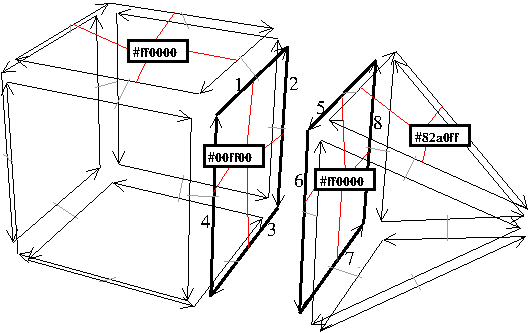
\includegraphics[width=\LargFig]{Combinatorial_map/fig/pdf/exemple-carte-3d-sew}\qquad
      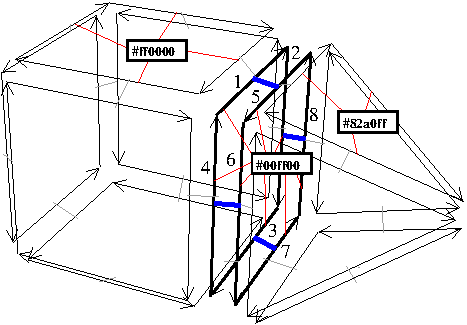
\includegraphics[width=\LargFig]{Combinatorial_map/fig/pdf/exemple-carte-3d-sew2}
    \end{center}
  \end{ccTexOnly}
  \begin{ccHtmlOnly}
    <CENTER> <A HREF="fig/png/exemple-carte-3d-sew.png"> <img
    src="fig/png/exemple-carte-3d-sew.png" alt=""></A> <A
    HREF="fig/png/exemple-carte-3d-sew2.png"> <img
    src="fig/png/exemple-carte-3d-sew2.png" alt=""></A> </CENTER>
  \end{ccHtmlOnly}
  \caption{Example of 3-sew operation. \textbf{Left}:~A 3D
    combinatorial map containing two volumes that are not connected,
    with 2-attributes. Each attribute contains a color in RGB format,
    and there are four 2-cells associated with attributes.
    Associations between darts and attributes are drawn with red
    segments. \textbf{Right}:~The 3D combinatorial map obtained as
    result of \ccc{sew<3>(1,5)} (or \ccc{sew<3>(2,8)}, or
    \ccc{sew<3>(3,7)}, or \ccc{sew<3>(4,6)}). Darts (1,5), (2,8),
    (3,7) and (4,6) are linked together by \betatrois{}. The two 2-cells
    \emph{c1}=\{1,2,3,4\} and \emph{c2}=\{5,6,7,8\} are merged after the sew
    into the 2-cell \{1,2,3,4,5,6,7,8\}. We are in the case where
    the two attributes are non NULL, thus the first one is kept, and
    all the darts of \emph{c2} are associated with the first attribute.}
  \label{fig-exemple-sew}
\end{figure}
%%%%%%%%%%%%%%%%%%%%%%%%%%%%%%%%%%%%%%%%%%%%%%%%%%%%%%%%%%%%%%%%%%%%%%%%%%%%%%
\begin{itemize}
\item The \ccc{sew} and \ccc{unsew} methods iterate over two orbits in
  order to link or unlink specific darts two by two.  Intuitively, a
  \ccc{sew<i>} operation glues two \cells{i} by identifying two of
  their \cells{(i-1)} (see example in Figure~\ref{fig-exemple-sew}
  where \ccc{sew<3>} is used to glue two 3-cells along one 2-cell).
  Reciprocally, a \ccc{unsew<i>} operation un-glues two \cells{i} which
  were glued along one of their \cells{(i-1)}.
  These methods guarantee that given a valid combinatorial map and a
  possible operation we obtain a valid combinatorial map as result of
  the operation.

\item
\begin{ccAdvanced}
  The \ccc{link_beta} and \ccc{unlink_beta} methods only modify
  the pointer of two darts: the obtained combinatorial maps may be not
  valid. These operations can be useful to use low level operations
  in a specific algorithm, for example to modify locally a
  combinatorial map in a really fast way. In such a case, additional
  operations may be needed to restore the validity conditions.
\end{ccAdvanced}
\end{itemize}

Linking two darts \emph{d1} and \emph{d2} by \betai{}, with 2\myleq{}\emph{i}\myleq{}\emph{d}
and \emph{d1}\myneq{}\emph{d2}, consists in modifying two \betai{} pointers such that
\betai{}(\emph{d1})=\emph{d2} and \betai{}(\emph{d2})=\emph{d1}. For \emph{i}=1, the modification
is \betaun{}(\emph{d1})=\emph{d2} (and thus \betazero{}(\emph{d2})=\emph{d1} by definition of
\betazero{}); in this case we can have \emph{d1=d2} (a dart linked with
itself corresponds to an edge which is a loop).

Reciprocally, unlinking a given dart \emph{d0} by \betai{}, with 2\myleq{}
\emph{i}\myleq{}\emph{d}, consists in modifying two \betai{} pointers
such that \betai{}(\betai{}(\emph{d0}))=$\varnothing$ and
\betai{}(\emph{d0})=$\varnothing$.  For \emph{i=1}, the modification is
\betaun{}(\emph{d0})=$\varnothing$ (and thus
\betazero{}(\betaun{}(\emph{d0}))=$\varnothing$ by definition of \betazero{}).  Note
that is it possible to unlink a given dart for \betai{} only if it is
not \emph{i}-free.

The \ccc{sew<i>(dh1,dh2)} method consists mainly to link two by two
several darts by \betai{}. This operation is possible only if there is
a bijection \emph{f} between all the darts of the orbit
\emph{D1}=\orbit{\betaun{},\myldots{},\betaimdeux{},\betaipdeux{},\myldots{},\betad{}}(\emph{d1}) and
\emph{D2}=\orbit{\betaun{},\myldots{},\betaimdeux{},\betaipdeux{},\myldots{},\betad{}}(\emph{d2})
satisfying: \emph{f}(\emph{d1})=\emph{d2}, and for all \emph{e}\myin{}\emph{D1}, 
for all \emph{j}\myin{}\{1,\myldots{},i-2,i+2,\myldots{},\emph{d}\},
\emph{f}(\betaj{}(\emph{e}))=\betajinv{}(\emph{f}(\emph{e})).  Intuitively, this condition
ensures the validity of the combinatorial map by verifying that
condition discussed in Section~\ref{ssec-combimap-validity} will be
satisfied after the operation.  This condition can be tested by using the method
\ccc{is_sewable<i>(dh1,dh2)}. For example, the function
\ccc{is_sewable<i>} would return \ccc{false} if we tried to sew a
triangular facet with a quad facet. Note that given two darts \emph{d1}
and \emph{d2}, if there is such a bijection, it is uniquely defined. So giving
the two darts as arguments of the \ccc{sew<i>} is enough to retrieve
all the pairs of darts to link.
If such a bijection exists, the \ccc{sew<i>(dh1,dh2)} operation
consists only in linking by \betai{} each couple of darts \emph{d3} and
\emph{d4} such that \emph{d3}=\emph{f}(\emph{d4}).

In addition, the sew operation updates the associations between darts
and non void attributes in order to guarantee that all the darts
belonging to a given cell are associated with the same attribute
(which is a condition of combinatorial map validity).  For each couple
of \cells{j} \emph{c1} and \emph{c2} that are merged into one \cell{j} during
the sew, we have to update the two associated attributes \emph{attr1} and
\emph{attr2}.  If both are NULL, there is nothing to do.  If one is NULL
and the other not, we only associate the non NULL attribute to all the
darts of the resulting cell.  When the two attributes are non NULL, we
first apply functor \ccc{On_merge} on the two attributes \emph{attr1} and
\emph{attr2} (see Section~\ref{ssec-attributes}). Then, we associate the
attribute \emph{attr1} to all darts of the resulting \cell{j}. Finally,
attribute \emph{attr2} is removed from the combinatorial map. 

Note that when the two attributes are non NULL, the first one is
kept. But user can customize this behavior in order to update the
information contained in the attributes according to its needs.  For
that, we can define a specific functor, and use it as template
argument for \ccc{OnMerge} parameter of the \ccc{Cell_attribute}
definition. This functor can for example copy the information of the
second attribute in the information of the first one to make as if the
second attribute is kept.

For example, in Figure~\ref{fig-exemple-sew}, we want to 3-sew the two
initial volumes. \ccc{sew<3>(1,5)} links by \betatrois{} the pairs of
darts (1,5), (2,8), (3,7) and (4,6), thus the combinatorial map
obtained is valid. 2-attributes are updated so that all the darts
belonging to the 2-cell containing dart 1 become associated to the
same 2-attribute after the operation.

Similarly, \ccc{unsew<i>(dh0)} operation unlinks \betai{} for all the darts
in the orbit 
\orbit{\betaun{},\myldots{},\betaimdeux{},\betaipdeux{},\myldots{},\betad{}}(\emph{d0}), 
and thus guarantees to obtain a valid combinatorial map.  This
operation is possible for any non \emph{i}-free dart.

As for the sew operations, attributes are updated to
guarantee that two darts belonging to two different \cells{j} are
associated to two different \emph{j}-attributes.  If the unsew operation
splits a \cell{j} \emph{c} in two \cells{j} \emph{c1} and \emph{c2}, and if \emph{c} is
associated to a \emph{j}-attribute \emph{attr1}, then this attribute is duplicated
into \emph{attr2}, and all the darts belonging to \emph{c2} are associated
with this new attribute.  Finally, we call the functor \ccc{On_split}
on the two attributes \emph{attr1} and \emph{attr2} (see
Section~\ref{ssec-attributes}).

Let us consider the combinatorial map given in
Figure~\ref{fig-exemple-sew} (Right). If we call \ccc{unsew<3>(2)}, we
obtain the combinatorial map in Figure~\ref{fig-exemple-sew} (Left)
(except for the color of the attribute associated to the
2-cell \{5,6,7,8\} which would be \texttt{\#00ff00}).  The \ccc{unsew<3>}
operation has duplicated the 2-attribute associated to the 2-cell
\{1,2,3,4,5,6,7,8\} since this 2-cell is split in two after the
unsew operation.

\begin{ccAdvanced}
  If one wants to modify a combinatorial map \emph{manually}, it is 
  possible to switch off the updating between
  darts and attributes by passing \ccc{false} as last argument of
  \ccc{sew<i>(dh1,dh2,update_attributes=true)} and
  \ccc{unsew<i>(dh0,update_attributes=true)}.  In these cases, the
  combinatorial map obtained may be no longer valid due to incorrect
  associations between darts and attributes.
  
  In Figure~\ref{fig-exemple-sew} (Left), if we call
  \ccc{sew<3>(1,5,false)}, the resulting combinatorial map is similar
  to the combinatorial map of Figure~\ref{fig-exemple-sew} (Right)
  (we have linked by \betatrois{} the pairs of darts (1,5), (2,8),
  (3,7) and (4,6)), but associations between darts and attributes
  are not valid. Indeed, we have kept the four initial attributes
  and all the associations between darts and attributes, thus two
  darts belonging to the same 2-cell (for example darts 1 and 5) are
  associated with two different attributes.

  We can also use the
  \ccc{link_beta<i>(dh1,dh2,update_attributes=true)} which links
  \ccc{d1} and \ccc{d2} by \betai{} without modifying the other
  links.
  Association between darts and attributes are only modified for darts
  \ccc{d1} and \ccc{d2}, and similarly as for \ccc{sew<i>}, this
  updating can be avoided by passing \ccc{false} as last argument of
  \ccc{link_beta<i>(dh1,dh2,update_attributes)}.  Lastly, we can use
  \ccc{unlink_beta<i>(dh0)} to unlink \ccc{d0} for \betai{}. In this
  last case, there is no modification of association between darts and
  attributes.

  In Figure~\ref{fig-exemple-sew} (Left), if we call
  \ccc{link_beta<3>(1,5)}, in the resulting combinatorial map we have
  now \betatrois{}(1)=5 and \betatrois{}(5)=1. This combinatorial map is no
  longer valid (for example dart 2 is 3-free and we should have
  \betatrois{}(2)=8).

\end{ccAdvanced}

\subsection{Removal and Insertion Operations}\label{ssec-operations}

The following high level operations are defined as global functions
taking an instance \ccc{cm} of \ccc{CombinatorialMap} as first
argument.  All these methods ensure that given a valid combinatorial
map and a possible operation, the modified combinatorial map is also
valid.

The first one is \ccc{remove_cell<CMap,i>(cm,dh0)} which modifies the
combinatorial map to remove the \cell{i} containing dart \ccc{d0},
with 0\myleq{}\emph{i}\myleq{}\emph{d}. This operation is possible 
if \emph{i}=\emph{d} or if the given
\cell{i} is incident to at most two \cells{(i+1)} which can be tested
thanks to \ccc{is_removable<CMap,i>(cm,dh0)}.  If the removed \cell{i}
was incident to two different \cells{(i+1)}, these two cells are
merged into one \cell{(i+1)}. In this case, the \ccc{On_merge} functor
is called if two \emph{(i+1)}-attributes are associated to the two
\cells{(i+1)}.  If the \cell{i} is associated with a non void
attribute, it is removed from the combinatorial map  (see three
examples on Figures~\ref{fig-insert-vertex}, \ref{fig-insert-edge} and
\ref{fig-insert-face}).

\begin{figure}[htb]
  \begin{ccTexOnly}
    \begin{center}
      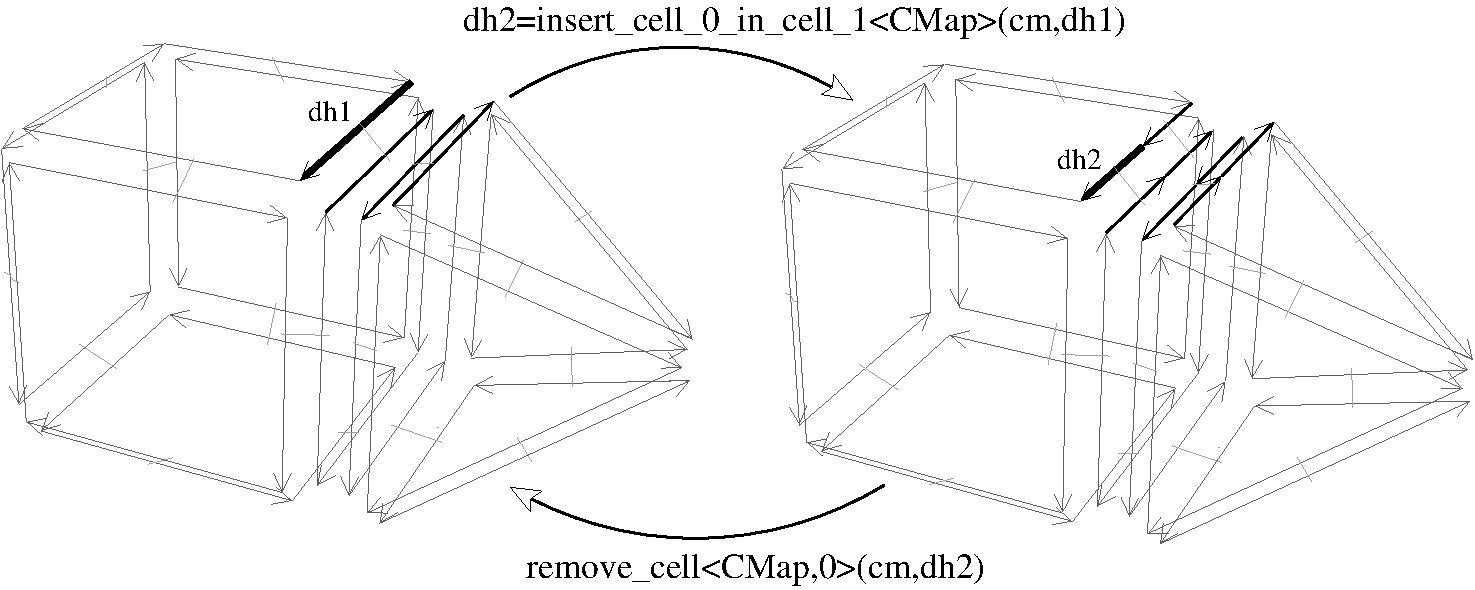
\includegraphics[width=.75\textwidth]{Combinatorial_map/fig/pdf/insert-vertex}
    \end{center}
  \end{ccTexOnly}
  \begin{ccHtmlOnly}
    <CENTER> <A HREF="fig/png/insert-vertex.png"><img
    src="fig/png/insert-vertex.png" alt=""></A> </CENTER>
  \end{ccHtmlOnly}
  \caption{Example of \ccc{insert_cell_0_in_cell_1} and
    \ccc{remove_cell<0>} operations. \textbf{Left}:~Initial
    combinatorial map.  \textbf{Right}:~After the insertion of a
    0-cell in the 1-cell containing dart \ccc{d1}.  Now if we remove
    the 0-cell containing dart \ccc{d2}, we obtain the initial
    combinatorial map.}
  \label{fig-insert-vertex}
\end{figure}

The inverse operation of the removal is the insertion operation.
Several versions exist, sharing a common principle. They consist in
adding a new \cell{i} "inside" an existing \cell{j}, \emph{i}\mylt{}\emph{j}, by
splitting the \cell{j} into several \cells{j}.  Contrary to
\ccc{remove_cell<CMap,i>}, is it not possible to define a unique
\ccc{insert_cell_i_in_cell_j<CMap,i,j>} function because parameters
are different depending on \ccc{i} and \ccc{j}.

\ccc{insert_cell_0_in_cell_1<CMap>(cm,dh0)} adds a 0-cell in
the 1-cell containing dart \ccc{d0}. The 1-cell is split in two. This
operation is possible if \ccc{d0}\myin{}\ccc{cm.darts()} (see
example on Figure~\ref{fig-insert-vertex}).

\ccc{insert_cell_0_in_cell_2<CMap>(cm,dh0)} adds a 0-cell in
the 2-cell containing dart \ccc{d0}. The 2-cell is split in
triangles, one for each initial edge of the facet. This operation
is possible if \ccc{d0}\myin{}\ccc{cm.darts()} (see example on
Figure~\ref{fig-triangulate}).

\begin{figure}[htb]
  \begin{ccTexOnly}
    \centerline{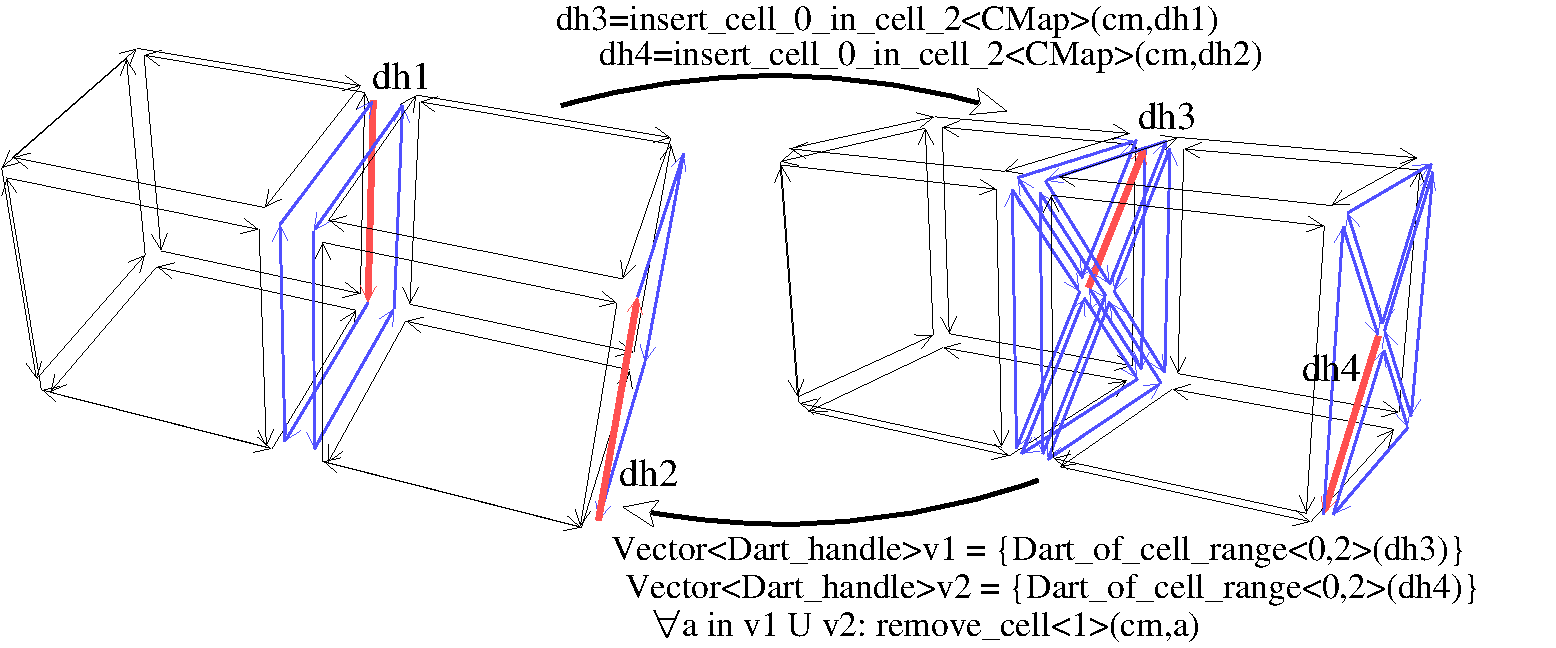
\includegraphics[width=.85\textwidth]
      {Combinatorial_map/fig/pdf/triangulation}}
  \end{ccTexOnly}
  \begin{ccHtmlOnly}
    <CENTER> <A HREF="fig/png/triangulation.png"> <img
    src="fig/png/triangulation.png" alt=""></A> </CENTER>
  \end{ccHtmlOnly}
  \caption{Example of \ccc{insert_cell_0_in_cell_2} operation.}
  \label{fig-triangulate}
\end{figure}

\ccc{insert_cell_1_in_cell_2<CMap>(cm,dh1,dh2)} adds a 1-cell in
the 2-cell containing darts \ccc{d1} and \ccc{d2}, between the two
0-cells containing darts \ccc{d1} and \ccc{d2}. The 2-cell is split
in two. This operation is possible if \emph{d1}\myin{}\orbit{\betaun{}}(\emph{d2})
which can be tested thanks to
\ccc{is_insertable_cell_1_in_cell_2(cm,dh1,dh2)}.  In the example on
Figure~\ref{fig-insert-edge}, it is possible to insert an edge
between darts \emph{d2} and \emph{d3}, but it is
not possible to insert an edge between \emph{d1} and \emph{d3}.

\begin{figure}[htb]
  \begin{ccTexOnly}
    \begin{center}
      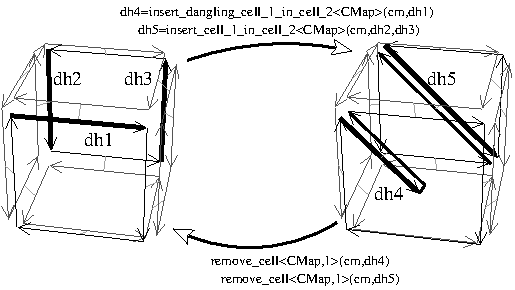
\includegraphics[width=.72\textwidth]{Combinatorial_map/fig/pdf/insert-edge}
    \end{center}
  \end{ccTexOnly}
  \begin{ccHtmlOnly}
    <CENTER> <A HREF="fig/png/insert-edge.png"><img
    src="fig/png/insert-edge.png" alt=""></A> </CENTER>
  \end{ccHtmlOnly}
  \caption{Example of \ccc{insert_cell_1_in_cell_2} and
    \ccc{remove_cell<1>} operations. \textbf{Left}:~Initial
    combinatorial map.  \textbf{Right}:~After the insertion of two
    1-cells: a first one between the two 0-cells containing darts
    \ccc{d2} and \ccc{d3}, and a second one incident to the 0-cell
    containing dart \ccc{d1}. Now if we remove the two
    1-cells containing darts \ccc{d4} and \ccc{d5}, we obtain the
    initial combinatorial map.}
  \label{fig-insert-edge}
\end{figure}


\ccc{insert_dangling_cell_1_in_cell_2<CMap>(cm,dh0)} adds a 1-cell in
the 2-cell containing dart \ccc{d0}, the 1-cell being attached by only
one of its vertex to the 0-cell containing dart \ccc{d0}.
This operation is possible if \ccc{d0}\myin{}\ccc{cm.darts()}.

\ccc{insert_cell_2_in_cell_3<CMap>(cm,itbegin,itend)} adds a
2-cell in the 3-cell containing all the darts between
\ccc{itbegin} and \ccc{itend}, along the path of 1-cells
containing darts in [\ccc{itbegin},\ccc{itend}). The 3-cell is
split in two. This operation is possible if all the 
darts in [\ccc{itbegin},\ccc{itend}) form a closed path inside a same 3-cell 
which can be tested thanks to
\ccc{is_insertable_cell_2_in_cell_3(cm,itbegin,itend)}
(see example on Figure~\ref{fig-insert-face}).

\begin{figure}[htb]
  \begin{ccTexOnly}
    \begin{center}
      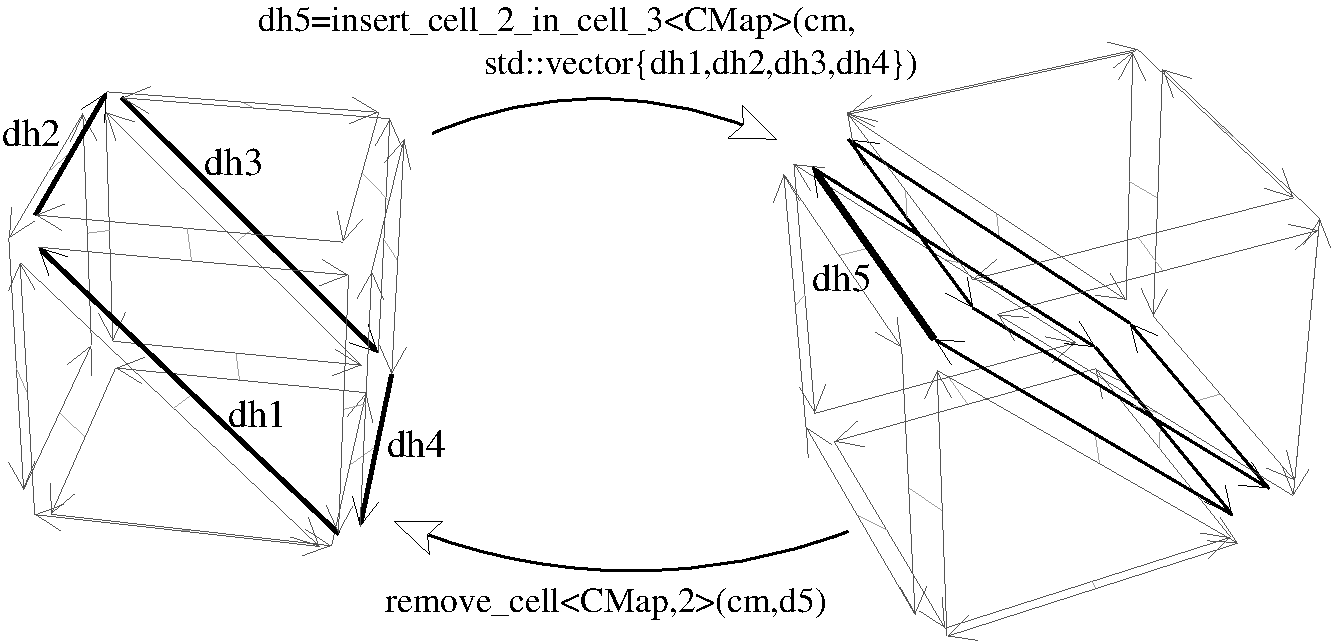
\includegraphics[width=.75\textwidth]{Combinatorial_map/fig/pdf/insert-facet}
    \end{center}
  \end{ccTexOnly}
  \begin{ccHtmlOnly}
    <CENTER> <A HREF="fig/png/insert-facet.png"><img
    src="fig/png/insert-facet.png" alt=""></A> </CENTER>
  \end{ccHtmlOnly}
  \caption{Example of \ccc{insert_cell_2_in_cell_3} and
    \ccc{remove_cell<2>} operations. \textbf{Left}:~Initial
    combinatorial map.  \textbf{Right}:~After the insertion of a
    2-cell along the path of 1-cells containing respectively
    \ccc{d1,d2,d3,d4}.  Now if we remove the 2-cell containing dart
    \ccc{d5}, we obtain the initial combinatorial map.}
  \label{fig-insert-face}
\end{figure}

Some examples of use of these operations are given in
Section~\ref{ssec-exemple-operations}.

\section{Examples}

\subsection{A 3D Combinatorial Map}\label{ssec-example-3DCM}

In this example, a 3-dimensional combinatorial map is constructed. Two
combinatorial tetrahedra are created, then the numbers of cells of the
combinatorial map are displayed, and the validity of the combinatorial
map is checked.  Then, we illustrate the use of ranges to iterate over
specific darts.  The first loop enumerates all the darts of the first
tetrahedron by using the range \ccc{Dart_of_orbit_range<1,2>}, and the
second loop enumerates all the darts of the facet containing dart
\ccc{dh2} by using the range
\ccc{Dart_of_orbit_range<1>}.

\ccIncludeExampleCode{Combinatorial_map/map_3_simple_example.cpp}

The output is:
\begin{verbatim}
#Darts=24, #0-cells=8, #1-cells=12, #2-cells=8, #3-cells=2, #ccs=2, valid=1
Number of darts of the first tetrahedron: 12
Number of darts of the facet containing dh2: 3
\end{verbatim}

which gives the number of darts of the combinatorial map, the numbers
of different cells, the number of connected components, and finally a
Boolean showing the validity of the combinatorial map (a tetrahedron
is made up of 12 darts because there are 3 darts per facet and there
are 4 facets).

%\begin{ccAdvanced}
Note the creation in the for loops of the two instances of
\ccc{Dart_of_orbit_range::const_iterator}: \ccc{it} is the current iterator,
and \ccc{itend} an iterator to the end of the range. Having
\ccc{itend} avoids calling \ccc{cm.darts_of_orbit<1,2>(dh1).end()}
again and again as in the following example (which is a bad
solution):
\begin{ccExampleCode}
  for (CMap_3::Dart_of_orbit_range<1,2>::const_iterator 
       it(cm.darts_of_orbit<1,2>(dh1).begin());
       it!=cm.darts_of_orbit<1,2>(dh1).end()); ++it)
  {...}
\end{ccExampleCode}
%\end{ccAdvanced}

\subsection{High Level Operations}
\label{ssec-exemple-operations}

This example shows some uses of high level operations.  First we
create a combinatorial hexahedron, the combinatorial map obtained is shown in
Figure~\ref{fig_exemple_ope} (Left). Then we insert two 1-cells along
two opposite 2-cells of the hexahedron. The combinatorial map
obtained is shown in Figure~\ref{fig_exemple_ope} (Middle).  Finally, we
insert a 2-cell in the diagonal of the hexahedron in order to split
it into two parts. We obtain the combinatorial map shown in
Figure~\ref{fig_exemple_ope} (Right). We display the characteristics
of the combinatorial map and check its validity.

The second part of this example removes the inserted elements. First
we remove the inserted 2-cell, then the two inserted 1-cells. We get
back the initial combinatorial hexahedron, which is verified by displaying once
again the characteristics of the combinatorial map.

\ccIncludeExampleCode{Combinatorial_map/map_3_operations.cpp}

The output is:
\begin{verbatim}
#Darts=36, #0-cells=8, #1-cells=14, #2-cells=9, #3-cells=2, #ccs=1, valid=1
#Darts=24, #0-cells=8, #1-cells=12, #2-cells=6, #3-cells=1, #ccs=1, valid=1
\end{verbatim}

The first line gives the characteristics of the combinatorial map
after all the insertions (the combinatorial map drawn in
Figure~\ref{fig_exemple_ope} (Right)). There are two 3-cells (since
the combinatorial hexahedron was split in two by the 2-cell
insertion), nine 2-cells (since two 2-cells of the original hexahedron
were split in two by the two 1-cell insertions, and a new 2-cell was
created during the 2-cell insertion), fourteen 1-cells (since there
are two new 1-cells created by the 1-cell insertion) while the number
of 0-cells remains unchanged.

The second line is the result after the removal operations. We
retrieve the original combinatorial hexahedron since we have removed
all the inserted elements.

%
%%%%%%%%%%%%%%%%%%%%%%%%%%%%%%%%% FIGURE %%%%%%%%%%%%%%%%%%%%%%%%%%%%%%%%%%%%%%%
\def\largFig{.25\textwidth}%
\begin{figure}
  \begin{ccTexOnly}
    \begin{center}
      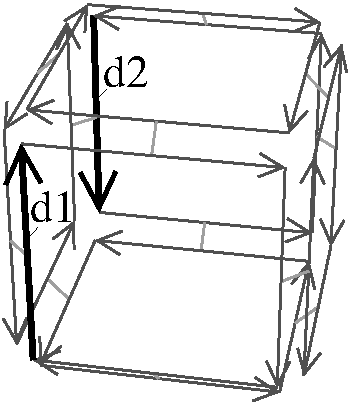
\includegraphics[width=\largFig]{Combinatorial_map/fig/pdf/ope1}\qquad
      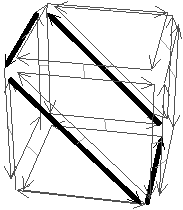
\includegraphics[width=\largFig]{Combinatorial_map/fig/pdf/ope2}\qquad
      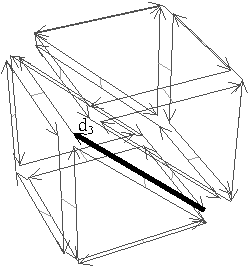
\includegraphics[width=\largFig]{Combinatorial_map/fig/pdf/ope3}
    \end{center}
  \end{ccTexOnly}
  \begin{ccHtmlOnly}
    <CENTER>
    <A HREF="fig/png/ope1.png"> <img src="fig/png/ope1.png" alt=""></A>
    <A HREF="fig/png/ope2.png"> <img src="fig/png/ope2.png" alt=""></A>
    <A HREF="fig/png/ope3.png"> <img src="fig/png/ope3.png" alt=""></A>
    </CENTER>
    \end{ccHtmlOnly}  
      \caption{Example of high level operations.  
        \textbf{Left}:~Initial 3D combinatorial map after the 
        creation of the combinatorial hexahedron.
        \textbf{Middle}:~Combinatorial map obtained after
        the two 1-cell insertions. The two 2-cells were split in two.
        \textbf{Right}:~Combinatorial map obtained after the 2-cell 
        insertion. The 3-cell was split in two.}
    \label{fig_exemple_ope}
\end{figure}
%%%%%%%%%%%%%%%%%%%%%%%%%%%%%%%%% FIGURE %%%%%%%%%%%%%%%%%%%%%%%%%%%%%%%%%%%%%%%


\subsection{A 4D Combinatorial Map}

In this example, a 4-dimensional combinatorial map is used.  Two
tetrahedral cells are created and sewn by \betaquatre{}.  Then the numbers
of cells of the combinatorial map are displayed, and its validity is
checked. 

By looking at these numbers of cells, we can see that the 4D
combinatorial map contains only one 3-cell. Indeed, the \ccc{sew<4>}
operation has identified by pairs all the darts of the two 3-cells
by definition of the sew operation (see Section~\ref{ssec-link-darts})
which, in 4D, links by \betatrois{} all the darts in
\orbit{\betaun{},\betadeux{}}(\emph{d1}) and in 
\orbit{\betaun{},\betadeux{}}(\emph{d2}).  The
situation is similar (but in higher dimension) to the
configuration where we have two triangles in a 3D combinatorial map,
and you use \ccc{sew<3>} between these two triangles. The two triangles
are identified since all their darts are linked by \betatrois{}, thus we
obtain a 3D combinatorial map containing only one 3-cell. Note that
this 3-cell is unbounded since the darts of the two triangles are all
2-free. In the 4D case, the 4-cell is unbounded since all its darts
are 3-free.

In this example, we also illustrate how to use the basic methods to
build "by hand" some specific configuration in a combinatorial
map. In fact, these functions are already present in the package:
function \ccc{make_triangle(cm)} is equivalent to
\ccc{CGAL::make_combinatorial_polygon(cm,3)} and
\ccc{make_tetrahedron(cm)} is equivalent to
\ccc{CGAL::make_combinatorial_tetrahedron(cm)}.  If we want to create a 4D
simplex, we must create five 3D simplexes, and sew them correctly
two by two by \betatrois{} (and so on if you want to create higher
dimensional combinatorial map).

\ccIncludeExampleCode{Combinatorial_map/map_4_simple_example.cpp}

The output is:
\begin{verbatim}
#Darts=24, #0-cells=4, #1-cells=6, #2-cells=4, #3-cells=1, #4-cells=2, #ccs=1, valid=1
\end{verbatim}

\subsection{Combinatorial Map With Attributes}
\label{ssec-combi-map-with-color}

In the following example, we illustrate how to specify the
2-attributes in a 3D combinatorial map. For that, we define our own
item class using \ccc{CGAL::Dart<3,CMap>} as type of dart, and
\ccc{CGAL::Cell_attribute<CMap,int,CGAL::Tag_true,Sum_functor,Divide_by_two_functor>} 
as attributes which contain an \ccc{int} and which are associated to
2-cells of the combinatorial map.

Functors \ccc{Sum_functor} and \ccc{Divide_by_two_functor} define a
custom behavior: when two attributes \ccc{ca1} and \ccc{ca2} are
merged into \ccc{ca1}, the value of \ccc{ca1} is the sum of the
two initial values.  When an attribute \ccc{ca1} is split in the two
attributes \ccc{ca1} and \ccc{ca2}, the value of each attribute is
half of the first value.

\ccIncludeExampleCode{Combinatorial_map/map_3_with_colored_facets.cpp}

The output is:
\begin{verbatim}
20; 7; 7; 7; 7; 7; 13; 13; 13; 13; 13; 
2; 7; 7; 7; 7; 7; 2; 13; 13; 13; 13; 13; 5; 10; 
#Darts=64, #0-cells=13, #1-cells=24, #2-cells=14, #3-cells=2, #ccs=1, valid=1
\end{verbatim}

Before the \ccc{cm.sew<3>}, each 2-cell of the first cube is
associated with an attribute having 7 as value, and each 2-cell of the
second cube with an attribute having 13 as value. During the
\ccc{cm.sew<3>}, two 2-cells are merged, thus the functor
\ccc{Sum_functor} is called on the two associated 2-attributes, and
the value of the new 2-cell is the sum of the two previous one: 20.

Then we call \ccc{CGAL::insert_cell_0_in_cell_2} on a dart which
belong to this 2-cell. This method splits the existing 2-cell in \emph{k}
2-cells, \emph{k} being the number of 1-cells of the initial 2-cell (4 in
this example). These splits are made consecutively, thus for the first
split, we create a new attribute as copy of the initial one and call
functor \ccc{Divide_by_two_functor} on these two attributes: the value
of each attribute is thus 20/2=10. For the second split, the value of
each attribute is thus 10/2=5, and for the last split the value of
each attribute is thus 5/2=2 (remember that information contained in
2-attributes in an \ccc{int}).  At the end, we obtain five
2-attributes with 7 as value, five 2-attributes with 13 as value, and
four 2-attributes having respectively 2, 2, 5 and 10 as values.

\section{Mathematical Definitions}\label{sec_definition}

The initial definition of combinatorial map in any dimension is given
in \cite{cgal:l-tmbrc-91,l-ndgcm-94}. But it allows only to represent
objects without boundaries. This definition was extended
\cite{cgal:pabl-cco-07,cgal:d-ccccg-10} in order to allow to represent 
objects with boundaries, based on the notions of partial permutations 
and partial involutions.

Intuitively, a \emph{partial permutation} on a finite set \emph{E} is a
mapping from \emph{E}\mycup{}\{$\varnothing$\} to \emph{E}\mycup{}\{$\varnothing$\} which is
injective on the subset of the domain that does not map to
$\varnothing$.  More precisely, a mapping \emph{p}: \emph{E}\mycup{}\{$\varnothing$\}
\myrightarrow{} \emph{E}\mycup{}\{$\varnothing$\} is a \emph{partial permutation}
defined on \emph{E} if:
\begin{enumerate}
\item \emph{p}($\varnothing$)=$\varnothing$;
\item \myforall{}\emph{e1}\myin{}\emph{E}, \myforall{}\emph{e2}\myin{}\emph{E},
  \emph{p}(\emph{e1})=\emph{p}(\emph{e2})\myneq{}$\varnothing$ \myRightarrow{} \emph{e1}=\emph{e2}.
\end{enumerate}

The inverse \pinv{} of this partial permutation is also a partial
permutation and is defined by:
\begin{enumerate}
\item \pinv{}($\varnothing$)=$\varnothing$;
\item \myforall{}\emph{e}\myin{}\emph{E}, if it exists \emph{a}\myin{}\emph{E} such that 
  \emph{p}(\emph{a})=\emph{e},
  then \pinv{}(\emph{e})=a, otherwise \pinv{}(\emph{e})=$\varnothing$.
\end{enumerate}

Let \emph{E} be a set, and \emph{p} a partial permutation on \emph{E}.  An element
\emph{e} is called a \emph{fixed point} for \emph{p} if \emph{p(e)=e}.  \emph{p} is a
\emph{partial involution} if \myforall{}\emph{e}\myin{}\emph{E}: \emph{p}(\emph{e})\myneq{}$\varnothing$
\myRightarrow{} \emph{p}(\emph{p}(\emph{e}))=\emph{e}.

Now we can give the definition of a combinatorial map in any dimension.
Let \emph{d}\mygeq{}0. A \emph{d}-dimensional combinatorial map (or 
\emph{d}-map) is a (d+1)-tuple \emph{M}=(\emph{D},\betaun{},\myldots{},\betad{}) 
where:
\begin{enumerate}
\item \emph{D} is a finite set of darts;
\item \betaun{} is a partial permutation on \emph{D};
\item \myforall{}\emph{i}, 2\myleq{}\emph{i}\myleq{}\emph{d}, \betai{} is a
  partial involution on \emph{D} without fixed point;
\item\label{cond-composition} \myforall{}\emph{i}: 0\myleq{}\emph{i}\myleq{}\emph{d}-2,
  \myforall{}\emph{j}: 3\myleq{}\emph{j}\myleq{}\emph{d}, \emph{i}+2\myleq{}\emph{j},
  \betai{}\comp{}\betaj{} is a partial involution.
\end{enumerate}

A \emph{d}-dimensional combinatorial map represents a subdivision of an
orientable \emph{d}-dimensional quasi-manifold. A dart is an abstract element
which is only required to define partial permutations. The last line of
the definition fixes constraints which guarantee the topological
validity of the represented object, i.e., the fact that it is a
quasi-manifold. This definition allows us to verify the validity of a
given combinatorial map by checking if each item of the definition is
satisfied.

Given a set of partial permutations 
\emph{S}=\{\ccTexHtml{$f_1$}{f<sub>1</sub>},\myldots{},\ccTexHtml{$f_k$}{f<sub>k</sub>}\}, 
we denote by \orbit{\emph{S}} the \emph{permutation group} generated by
\{\ccTexHtml{$f_1$}{f<sub>1</sub>},\myldots{},\ccTexHtml{$f_k$}{f<sub>k</sub>}\} 
and whose group operation is the composition of partial permutations.  
The orbit \orbit{\ccTexHtml{$f_1$}{f<sub>1</sub>},\myldots{},\ccTexHtml{$f_k$}{f<sub>k</sub>}}(\emph{a}) 
is the set of darts which can be obtained from \emph{a} by elements of \orbit{\emph{S}}:
\orbit{\ccTexHtml{$f_1$}{f<sub>1</sub>},\myldots{},\ccTexHtml{$f_k$}{f<sub>k</sub>}}(\emph{a})=\{\myphi{}(\emph{a})$|$\myphi{}\myin{}\orbit{\emph{S}}\}\mysetminus{}\{$\varnothing$\}.

Let \emph{d0}\myin{}\emph{D} be a dart. Given \emph{i}, 1\myleq{}\emph{i}\myleq{}\emph{d},
the \cell{i} containing \emph{d0} is 
\orbit{\betaun{},\myldots{},\betaimun{},\betaipun{},\myldots{},\betad{}}(\emph{d0}).
The \emph{0}-cell  containing \emph{d0} is 
\orbit{\{\betai{}\comp{}\betaj{}$|$\myforall{}\emph{i,j}: 1\myleq{}\emph{i}\mylt{}\emph{j}\myleq{}\emph{d}\}}(\emph{d0}).

\section{Design and Implementation History}

The code of this package is inspired by Moka, a 3D topological modeler
mainly developed by Fr\'ed\'eric Vidil and Guillaume Damiand
(\ccAnchor{http://moka-modeller.sourceforge.net/}{http://moka-modeller.sourceforge.net/}).
However, Moka was based on Generalized maps (and not Combinatorial
maps), and the design was not \cgal\ "compatible". Thus, Guillaume
Damiand started to develop a totally new package by mixing ideas taken
from Moka with the design of the Halfedge data structure package of
\cgal.  Andreas Fabri and S\'ebastien Loriot contributed to the
design, the coding, and to the documentation of the package, and
Laurent Rineau helped for the design. Emma Michel contributed to the
manual. Monique Teillaud and Bernd Gaertner contributed to the manual
by giving useful remarks, really numerous and detailed for Monique.
